\section{考察}
前章では干渉パターンを4つの要素に分解し、位相に関係した2つのパラメータ$B, C$については実験結果を理論がよく説明することを見た。しかし波の水深に関係した2つのパラメータ$A, D$については実験結果と理論との間に相違が見られた。この章ではこの相違を説明するために2つの異なる仮説を立て、それぞれ仮説の下で実験結果がうまく説明できるかを考察する。

\subsection{スピンフリッパー間の距離による効果}
位相の異なる波が重ね合わさるとうなりが生じ振幅は変動する。これまでの議論では波長によって変化する位相、すなわち分散性位相は小さく、十分小さい波長領域でみる限りは振幅への影響はほとんどなかった。しかしもし考慮していない効果によって大きな分散性位相が生じるとすれば、振幅への影響は大きなものとなり、パラメータ$A$の実験結果をうまく説明できるかもしれない。

\paragraph{効果の取り入れ}
2つのスピンフリッパーが距離$L$だけ離れているとする。時刻$t$に上流側のフリッパーを通過した速度$v$の中性子は時刻$t+L/v$に下流側のフリッパーを通過する。中性子がスピンフリッパー間を飛行するのにかかる時間$L/v$の間にスピンフリッパーの振動磁場$2B_r\cos\omega_s t$の位相は$\omega_s L/v$だけまわってしまう。この効果を取り入れるために下流側のスピンフリッパーの振動磁場の位相を$\omega_s L/v$だけずらし、$2B_r\cos\omega_s (t+L/v)$としてみる。
\begin{figure}[h]
\centering
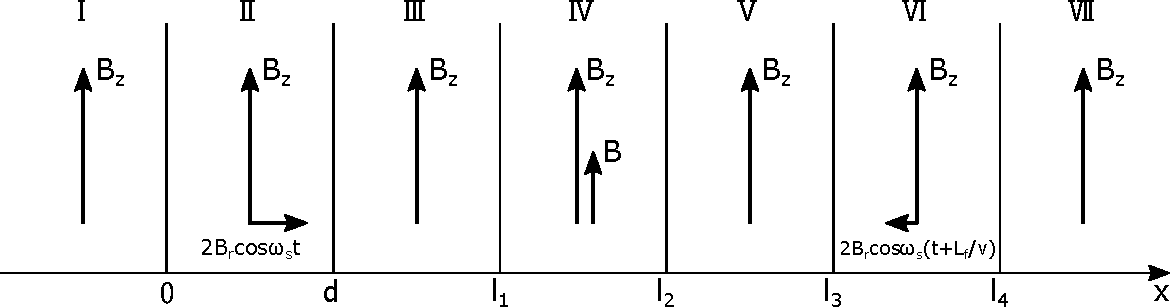
\includegraphics[height=3cm]{discussion/FD/FD_setting.pdf}
\end{figure}

\renewcommand{\arraystretch}{1.5}
簡単のため共鳴条件が満たされており、また2つのフリッパーで$\omega_r$が等しい場合を考えると、領域Iで
\begin{equation}
\psi_\mathrm{I}(x,t)=\begin{pmatrix} 1\\0\end{pmatrix} \e^{i (k_0-\frac{\omega_z}{v})x}\e^{-i\omega_0t}
\end{equation}
と表された入射中性子は領域VIIで
\begin{align}
&\psi_\mathrm{VII}(x,t) \notag \\
&=\scalebox{0.85}{$\begin{pmatrix} \cos \frac{\omega_rd}{v} & -i\sin\frac{\omega_rd}{v} \e^{-i\omega_s (t+\frac{L}{v})} \\ -i\sin\frac{\omega_rd}{v} \e^{-i\omega_s (t+\frac{L}{v})} &\cos \frac{\omega_r}{v}d\end{pmatrix} \begin{pmatrix} \e^{-i\frac{\omega d'}{v}} &0 \\0&\e^{i\frac{\omega d'}{v}} \end{pmatrix} \begin{pmatrix} \cos \frac{\omega_r d}{v} & -i\sin\frac{\omega_r d}{v} \e^{-i\omega_s t} \\ -i\sin\frac{\omega_r d}{v} \e^{-i\omega_s t} &\cos \frac{\omega_r d}{v}\end{pmatrix} \begin{pmatrix} 1\\0\end{pmatrix} \e^{i (k_0-\frac{\omega_z}{v})x}\e^{-i\omega_0t}$} \notag \\
&=\begin{pmatrix} \cos^2 \frac{\omega_r d}{v} \e^{-i\frac{\omega d'}{v}} -\sin^2 \frac{\omega_r d}{v} \e^{i\frac{\omega d'}{v}-i\frac{\omega_s L}{v}} \\ -i\sin\frac{\omega_r d}{v}\cos\frac{\omega_r d}{v}\left(\e^{-i\frac{\omega d'}{v} +i\frac{\omega_s L}{v}}+\e^{i\frac{\omega d'}{v}} \right) \e^{i\omega_s t} \end{pmatrix} \e^{i (k_0-\frac{\omega_z}{v})x}\e^{-i\omega_0t}
\end{align}
\renewcommand{\arraystretch}{1}
という状態をとる。従って領域VIIでスピン上向き中性子を観測する確率は
\begin{align}
|\psi_\mathrm{VII}^+|^2&=\left| \cos^2 \frac{\omega_r d}{v} \e^{-i\frac{\omega d'}{v}} -\sin^2 \frac{\omega_r d}{v} \e^{i\frac{\omega d'}{v}-i\frac{\omega_s L}{v}} \right|^2 \notag \\
&=\cos^4 \frac{\omega_r d}{v} +\sin^4 \frac{\omega_r d}{v}-\sin^2 \frac{\omega_r d}{v} \cos^2 \frac{\omega_r d}{v} \cos \left( \frac{2\omega d'}{v} -\frac{\omega_s L}{v} \right)
\end{align}
となって大きな分散性位相$-\omega_s L/v$が現れる。

必ずしも共鳴条件を満たさず、必ずしも2つのフリッパーで$\omega_r$が等しくない場合についても同様に、干渉パターンは式(\ref{analysis_N1r}), (\ref{analysis_N2r}), (\ref{analysis_N3r})の$N_1, N_2, N_3$を用いて
\begin{equation}
I=N_1-N_4\cos\left(\frac{2}{v} (\omega d' -\epsilon L') -\phi -\frac{\omega_s L}{v} \right)\label{Discussion_FD_theory_s}
\end{equation}
と書ける。ここで$N_4=\sqrt{N_2^2+N_3^2}, \cos\phi=N_2/N_4, \sin\phi=N_3/N_4$である。

\paragraph{結果}
次の図\ref{Discussion_FD_fig_s_470}は波長領域$\lambda=3.35\pm0.07$\AA における干渉パターンを式\ref{Discussion_FD_theory_s}を用いてフィッティングした結果である。フィッティングパラメータは$\epsilon/|\omega_z|$であり、図\ref{Discussion_FD_fig_s_470}のとき$\epsilon/|\omega_z|=0.112\pm0.001$、reduced$\chi^2=41.2/16=2.57$となった。振幅からのずれは十分小さく、振幅、位相共に実験値と理論値はよく一致している。しかし図\ref{Discussion_FD_fig_s}に表す他の波長領域で見ると位相がずれていることがわかる。なお各種パラメータには実測と測定データから求めた表\ref{analysis_tbl_parameter}, \ref{Discussion_FD_tbl_parameter}の値を用いた。
\begin{figure}[h]
\centering
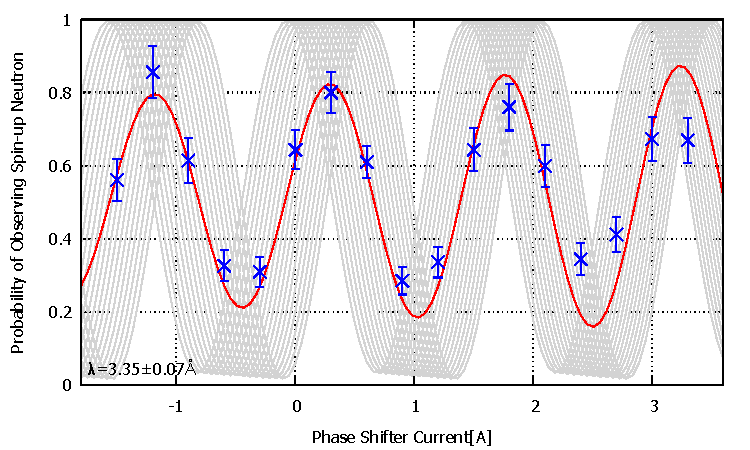
\includegraphics[width=10cm]{discussion/FD/IT_s_470.pdf}
\caption{波長領域$\lambda=3.35\pm0.07$\AA における干渉パターンのフィッティング結果\newline 青が実験結果、灰色が波長領域内での0.01\AA 毎の理論値、赤が波長領域内での理論値の積分を表す}\label{Discussion_FD_fig_s_470}
\end{figure}

\begin{table}[h]
\centering
\caption{各種パラメータ2}\label{Discussion_FD_tbl_parameter}
\begin{tabular}{cc}
$\omega_s/2\pi$[kHz]&$L$[mm]\\ \hline
$-37.5$&$403$
\end{tabular}
\end{table}

\begin{figure}[H]
\begin{minipage}{0.5\hsize}
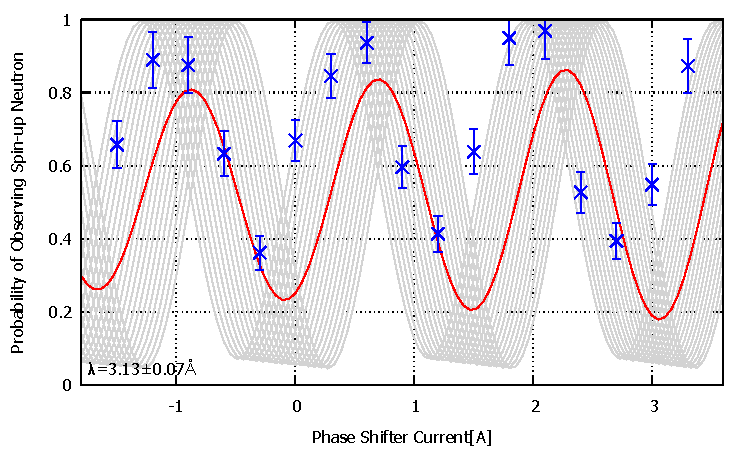
\includegraphics[width=\hsize]{discussion/FD/IT_s_440.pdf}
\end{minipage}
\begin{minipage}{0.5\hsize}
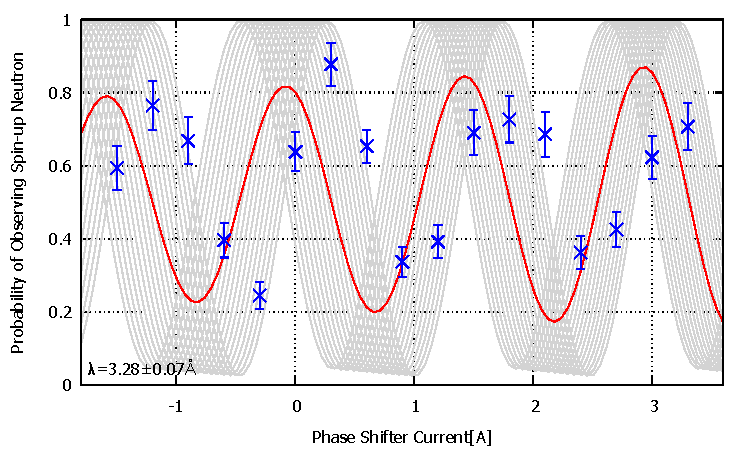
\includegraphics[width=\hsize]{discussion/FD/IT_s_460.pdf}
\end{minipage}\\
%\caption{様々な波長領域における干渉パターン}
%\end{figure}
%\begin{figure}[H]
%\ContinuedFloat
\begin{minipage}{0.5\hsize}
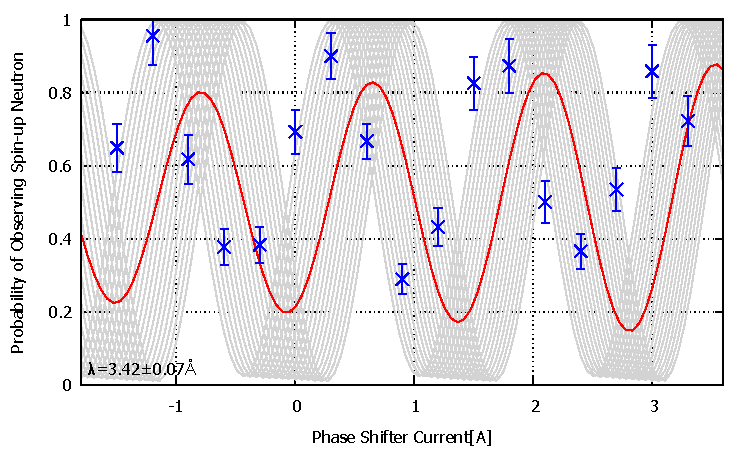
\includegraphics[width=\hsize]{discussion/FD/IT_s_480.pdf}
\end{minipage}
\begin{minipage}{0.5\hsize}
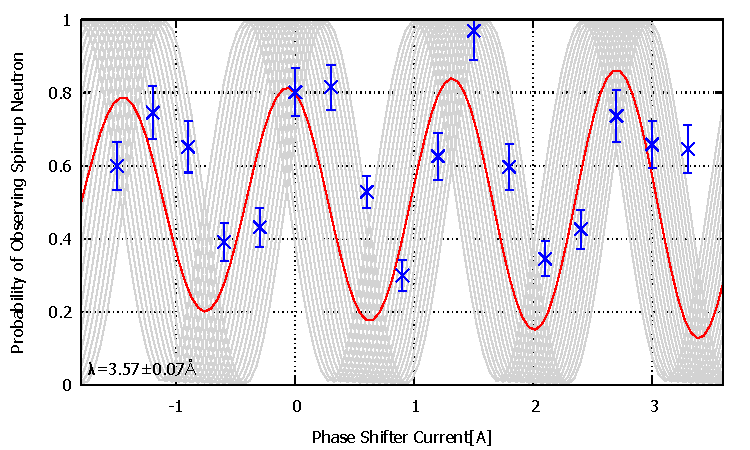
\includegraphics[width=\hsize]{discussion/FD/IT_s_500.pdf}
\end{minipage}
\caption{様々な波長領域における干渉パターン}\label{Discussion_FD_fig_s}
\end{figure}

\paragraph{解析}
前節で見たように、スピンフリッパー間の距離の効果を考慮すると、ある波長については振幅、位相共に実験値を理論値で説明することができたが、他の波長では位相にずれが生じた。そこで波を分解して、位相に関係するパラメータ$C$について解析する。

いまパラメータ$C$と理論的に対応する量は、式(\ref{Discussion_FD_theory_s})より
\begin{equation}
\frac{2\epsilon L'}{v} +\phi +\frac{\omega_s L}{v}+2n\pi \quad (n:整数)
\end{equation}
である。そこでパラメータ$C$の実験値と$\epsilon/|\omega_z|=0.112$のときの$n=10, 11, 12, 13, 14$における理論値を図\ref{Discussion_FD_fig_C_s_470_fit}に表す。
\begin{figure}[H]
\centering
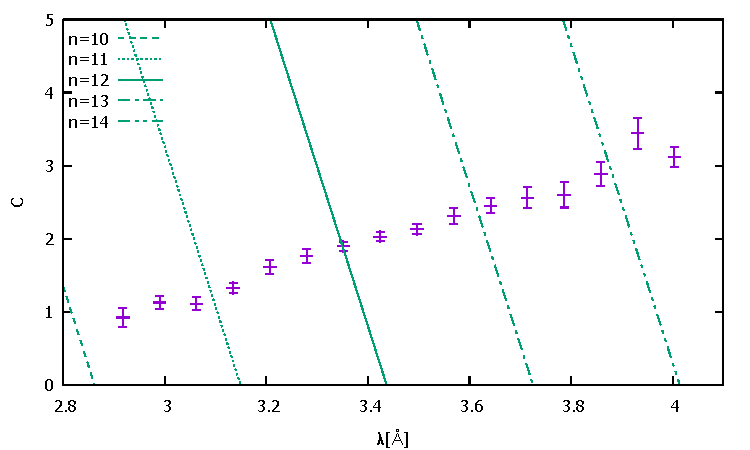
\includegraphics[width=9cm]{discussion/FD/C_s_470_fit.pdf}
\caption{パラメータ$C$の実験値と理論値}\label{Discussion_FD_fig_C_s_470_fit}
\end{figure}

このようにあるひとつの波長領域に対しては$\epsilon$を調節することでパラメータ$C$の実験値と理論値を合わせることができるが、大きな分散性位相$\omega_s L/v$のために他の波長領域ではどうしてもずれが生じる。
%逆に全ての波長領域でパラメータ$C$の実験値と理論値が合うためには大きな分散性位相を打ち消すほどの共鳴からのずれ$\epsilon/|\omega_z|=1$程度が必要となるが、共鳴実験からそれほど大きな共鳴からのずれは生じ得ないことが分かっている。
すなわち、スピンフリッパー間の距離のために生じた大きな分散性位相によって、十分小さな波長領域においても大きく位相のずれた波が重なり合い、うなりが生じて振幅が小さくなるという仮説は、パラメータ$C$の実験結果によって否定される。

\paragraph{考察}
\renewcommand{\arraystretch}{1.5}
中性子の波束としての取り扱いについて考え、なぜスピンフリッパー間の距離が実験結果に影響を与えないかを考察する。いま入射波束として次の形のものをとる:
\begin{equation}
\Psi_\mathrm{I}=\frac{1}{\sqrt{2\pi}}\int dk' g(k') \begin{pmatrix} 1\\ 0 \end{pmatrix} \e^{ik'x-i\omega'(k') t}
\end{equation}
ここで$g(k)$は中心$k=k_0$をもち、$k=k_0$から離れると速やかに減衰するある波数分布とする。また、$\omega'(k')=k'^2/2m+\omega_z$である。このとき群速度$v_g=d \omega'(k')/d k'|_{k'=k_0} =k_0/m$
\begin{comment}
\begin{equation}
群速度v_g=\frac{\del \omega'(k')}{\del k'} \Bigg|_{k'=k_0} =\frac{k_0}{m}
\end{equation}
\end{comment}
となる。
領域Iにおいて波束を形成する平面波
\begin{equation}
\begin{pmatrix} 1\\ 0 \end{pmatrix} \e^{ik'x-i\omega'(k') t}
\end{equation}
はそれぞれがShr$\ddot{\mathrm{o}}$dinger方程式に従って時間発展し、領域VIIでは
\begin{equation}
\begin{pmatrix} \cos^2 \frac{\omega_r d}{v'} \e^{-i\frac{\omega d'}{v'}} -\sin^2 \frac{\omega_r d}{v'} \e^{i\frac{\omega d'}{v'}} \\ -i\sin\frac{\omega_r d}{v'}\cos\frac{\omega_r d}{v'}\left(\e^{-i\frac{\omega d'}{v'}}+\e^{i\frac{\omega d'}{v'}} \right) \e^{i\omega_s t} \end{pmatrix} \e^{i k'x-i\omega'(k')t}
\end{equation}
となる。ここで$v'=\sqrt{(k'/m)^2+2\omega_z/m}$。ただし簡単のため共鳴条件が満たされており、2つのフリッパーで$\omega_r$は等しいとした。従って領域VIIにおける波束は次のように書ける:
\begin{equation}
\Psi_\mathrm{VII}=\frac{1}{\sqrt{2\pi}}\int dk' g(k') \begin{pmatrix} \cos^2 \frac{\omega_r d}{v'} \e^{-i\frac{\omega d'}{v'}} -\sin^2 \frac{\omega_r d}{v'} \e^{i\frac{\omega d'}{v'}} \\ -i\sin\frac{\omega_r d}{v'}\cos\frac{\omega_r d}{v'}\left(\e^{-i\frac{\omega d'}{v'}}+\e^{i\frac{\omega d'}{v'}} \right) \e^{i\omega_s t} \end{pmatrix} \e^{i k'x-i\omega'(k')t}
\end{equation}
つまり、スピンフリッパーによる位相は、波束そのものではなく波束を形成する平面波が受け取るものであり、波束中心の位置には依らない。よってスピンフリッパー間の距離は実験結果に影響を与えない。
\renewcommand{\arraystretch}{1}

いま$g(k)$として次の形:
\begin{equation}
g(k)=\frac{1}{\sqrt{\Delta} \pi^{\frac{1}{4}}} \exp \left[-\frac{1}{2\Delta^2}(k-k_0)^2\right]
\end{equation}
を考えると、領域VIIにおいてスピン上向き中性子を観測する確率は
\begin{equation}
|\Psi_\mathrm{VII}^+|^2=\left|\frac{1}{\sqrt{2\pi}}\int dk' \frac{1}{\sqrt{\Delta} \pi^{\frac{1}{4}}} \e^{ -\frac{1}{2\Delta^2}(k'-k_0)^2}\left( \cos^2 \frac{\omega_r d}{v'} \e^{-i\frac{\omega d'}{v'}} -\sin^2 \frac{\omega_r d}{v'} \e^{i\frac{\omega d'}{v'}} \right) \e^{i k'x-i\omega'(k')t} \right|^2
\end{equation}
となるが、幅$\Delta$が$k_0$に比べて十分狭ければ
\begin{align}
|\Psi_\mathrm{VII}^+|^2&\simeq \left| \cos^2 \frac{\omega_r d}{v_0} \e^{-i\frac{\omega d'}{v_0}} -\sin^2 \frac{\omega_r d}{v_0} \e^{i\frac{\omega d'}{v_0}} \right|^2 \left|\frac{1}{\sqrt{2\pi}}\int dk' \frac{1}{\sqrt{\Delta} \pi^{\frac{1}{4}}} \e^{ -\frac{1}{2\Delta^2}(k'-k_0)^2}\e^{i k'x-i\omega'(k')t} \right|^2 \notag \\
&=\left(\cos^4 \frac{\omega_r d}{v_0} +\sin^4 \frac{\omega_r d}{v_0}-\sin^2 \frac{\omega_r d}{v_0} \cos^2 \frac{\omega_r d}{v_0} \cos \frac{2\omega d'}{v_0} \right) \frac{1}{\sqrt{\left(\left(\frac{\Delta t}{m}\right)^2+\left(\frac{1}{\Delta}\right)^2\right)\pi}}\exp\left[-\frac{(x-v_0 t)^2}{\left(\frac{\Delta t}{m}\right)^2+\left(\frac{1}{\Delta}\right)^2}\right]
\end{align}
とできる。ここで$k_0^2/m \gg |\omega_z|$より$v_0=\sqrt{(k_0/m)^2+2\omega_z/m}\simeq k_0/m=v_g$を用いた。速度中心$v_0$をもつスピン上向き中性子波束を1個入射し、位置$x=X_d$に置いた検出器で検出することを考えると、十分早い時刻$t \ll m/\Delta^2$では波束の幅は一定と見なしてよいから、十分早い時刻$t$から$t+dt$の間にスピン上向き中性子を観測する確率は
\begin{equation}
P=\left(\cos^4 \frac{\omega_r d}{v_0} +\sin^4 \frac{\omega_r d}{v_0}-\sin^2 \frac{\omega_r d}{v_0} \cos^2 \frac{\omega_r d}{v_0} \cos \frac{2\omega d'}{v_0} \right) \frac{\Delta v_0dt}{\sqrt{\pi}}\exp\left[-\Delta^2(X_d-v_0 t)^2\right]
\end{equation}
となり、$t=X_d/v_0$を中心に幅$1/(\sqrt{2} v_0 \Delta)$で分布する。この幅が検出時間幅に対して小さければ、時刻$t=X_d/v_0$を含む検出時間幅でスピン上向き中性子を観測する確率は
\begin{align}
I&=\left(\cos^4 \frac{\omega_r d}{v_0} +\sin^4 \frac{\omega_r d}{v_0}-\sin^2 \frac{\omega_r d}{v_0} \cos^2 \frac{\omega_r d}{v_0} \cos \frac{2\omega d'}{v_0} \right) \int dt \frac{\Delta v_0}{\sqrt{\pi}}\exp\left[-\Delta^2(X_d-v_0 t)^2\right] \notag \\
&=\cos^4 \frac{\omega_r d}{v_0} +\sin^4 \frac{\omega_r d}{v_0}-\sin^2 \frac{\omega_r d}{v_0} \cos^2 \frac{\omega_r d}{v_0} \cos \frac{2\omega d'}{v_0}
\end{align}
となり、波束で考えたときの干渉パターンと平面波で考えたときの干渉パターンは一致する。

\subsection{バックグラウンド}
干渉を見る波長領域の中にミラーで反射されていない中性子が混ざっていたとすると、その分干渉波の振動中心は粒子数の多い方にずれ、観測確率として見たときの干渉波の振幅は小さくなることが予想される。

\paragraph{形}
バックグラウンドの分布としてどのような形を仮定するべきか検討を行う。次の図\ref{Discussion_fig_flipperoff}はスピンフリッパーをOFFにしたときの規格化粒子数の波長分布である。0\AA 付近に高速中性子の立ち上がりが、3.2\AA 付近に反射中性子のピークが見える。そしてその間1\AA 付近にもピークが確認できる。図\ref{Discussion_fig_mirroroff}はミラーを置かずに測定を行ったときの検出粒子数の波長分布であり、1\AA 付近のピークはKUANSからの熱中性子のピークである。すなわち図\ref{Discussion_fig_flipperoff}の1\AA 付近のピークはミラーで反射されずに検出された熱中性子の一部であると考えられる。
\begin{figure}[H]
%\begin{minipage}{0.5\hsize}
\centering
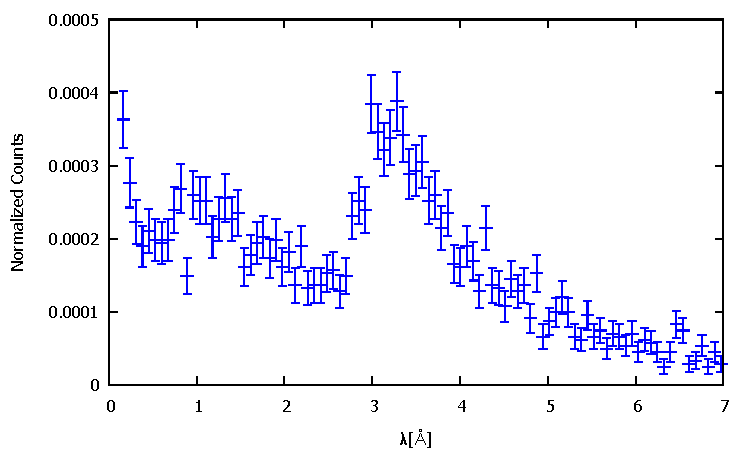
\includegraphics[width=9cm]{discussion/BG/flipperoff.pdf}
\caption{フリッパーOFF時の規格化粒子数波長分布(\ce{^3He}比例計数管による測定)}\label{Discussion_fig_flipperoff}
%\end{minipage}
\end{figure}
\begin{figure}[H]
%\begin{minipage}{0.5\hsize}
\centering
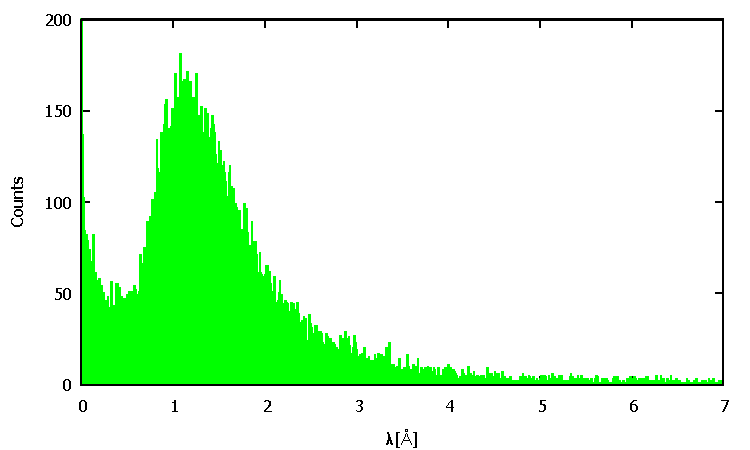
\includegraphics[width=9cm]{discussion/BG/mirroroff.pdf}
\caption{ミラーを置かずに測定した粒子数波長分布(RPMT検出器による測定)}\label{Discussion_fig_mirroroff}
%\end{minipage}
\end{figure}

%\newpage
次の図\ref{Discussion_fig_detectormove}はスピンフリッパーOFF時に検出器の$y$座標を、図\ref{Discussion_fig_flipperoff}の測定位置を$y=0$として、$y=-18, -9, 0, +9, +18$mmと動かしたときの規格化粒子数波長分布である。図\ref{Discussion_fig_detectormove}から$y=0$に近づくにつれ反射中性子のピークが大きくなっていくことがわかるが、5.5\AA 以上の長波長における分布は検出器の位置を動かしてもほとんど一定である。すなわち5.5\AA 以上の長波長においても消えない一定数のバックグラウンドが存在する。
\begin{figure}[h]
\begin{minipage}{0.5\hsize}
\centering
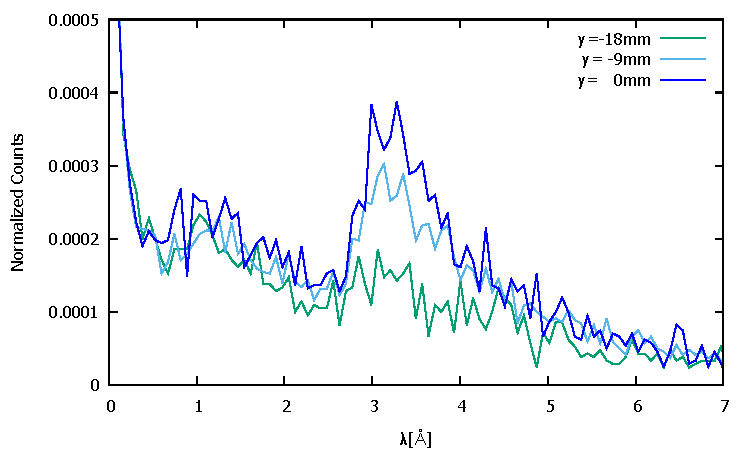
\includegraphics[width=\hsize]{discussion/BG/flippermove1.pdf}
\end{minipage}
\begin{minipage}{0.5\hsize}
\centering
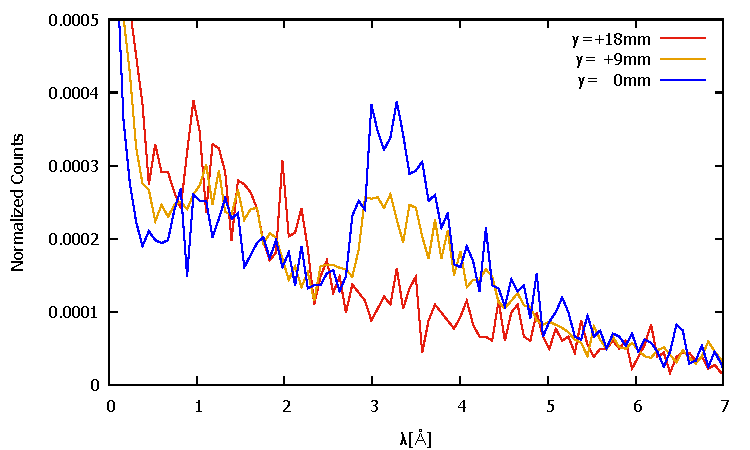
\includegraphics[width=\hsize]{discussion/BG/flippermove2.pdf}
\end{minipage}
\caption{検出器の位置を動かしたときの規格化粒子数}\label{Discussion_fig_detectormove}
\end{figure}

以上からバックグラウンドとしてあるピークを持ち長波長で消えないものを取りたい。そこで最もシンプルにガウシアンに定数項のついた$a\exp(-(x-b)^2/2c^2)+d$の形を採用する。なおもともとの熱中性子はMaxwell分布に従うが、バックグラウンドとして検出されたものは壁などで反射された成分などを含み元の分布とは異なると考えられるため、シンプルな形を採用した。図\ref{Discussion_fig_flipperoff}を反射成分を除く0.5-2.5と5.5-7\AA の範囲でフィッティングした結果を図\ref{Discussion_fig_backfit}に表し、各パラメータの値を表\ref{Discussion_tbl_backfit}に示す。

\begin{figure}[H]
\begin{minipage}{0.7\hsize}
\centering
%\vspace{2.5cm}
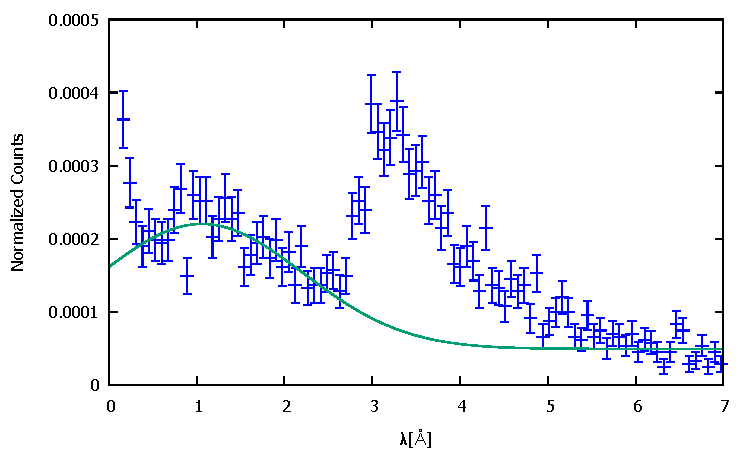
\includegraphics[width=10cm]{discussion/BG/background.pdf}
\caption{バックグラウンド} \label{Discussion_fig_backfit}
\end{minipage}
\begin{minipage}{0.3\hsize}
\centering
\makeatletter
\def\@captype{table}
\makeatother
\caption{各パラメータ} \label{Discussion_tbl_backfit}
\begin{tabular}{|c|c|} \hline
$a$&$1.7\times 10^{-4}\pm 1\times10^{-5}$\\ \hline
$b$&$1.1\pm0.2$\\ \hline
$c$&$1.1\pm0.2$\\ \hline
$d$&$4.9\times 10^{-5}\pm4\times 10^{-6}$\\ \hline
\end{tabular}
\end{minipage}
\end{figure}

\paragraph{結果}
\ref{phase_shifter_sec}章と同様に次の手順でバックグラウンドを考慮した場合のスピン上向き中性子観測確率の干渉パターンとフィッティングパラメータ$A, B, C, D$を得た。
\begin{enumerate}
\item シフタコイル電流を変えていったときの規格化粒子数の波長分布(図\ref{Discussion_fig_NC})からバックグラウンドを取り除いた分布(図\ref{Discussion_fig_NC_b})を得た
\item 図\ref{Discussion_fig_NC_b}の分布において種々の中心波長$\pm0.07$\AA の波長領域に含まれる規格化粒子数を数え、シフタコイル電流を横軸とした干渉パターン(図\ref{Discussion_fig_IF_nb})を得た
\item 干渉パターンを$-A'\cos(Bx+C)+D'$でフィットした
\item フリッパーOFF時の規格化粒子数からバックグラウンドを除いた分布から、そろぞれの波長領域における干渉パターンの縦軸(規格化粒子数)をスピン上向き中性子の観測確率とするためのファクターを求めた
\item 図\ref{Discussion_fig_IF_nb}を上で求めたファクターで割り、スピン上向き中性子の観測確率の干渉パターン(図\ref{Discussion_fig_IF_rb})を得た
\item フィッティングパラメータ$A', D'$をファクターで割り、理論と比較可能なパラメータ$A, B, C, D$を得た(表\ref{Discussion_tbl_IF_rb})
\end{enumerate}

\begin{figure}[h]
\begin{minipage}{0.33\hsize}
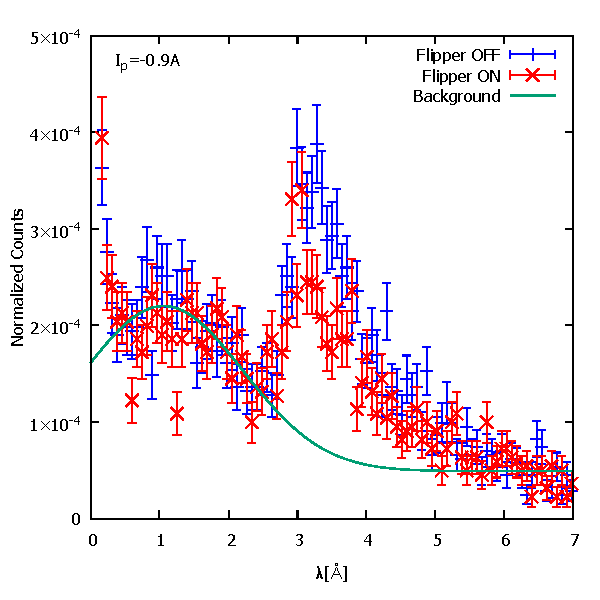
\includegraphics[width=5cm]{discussion/NC/NormalizedCounts_-9A.pdf}
\end{minipage}
\begin{minipage}{0.33\hsize}
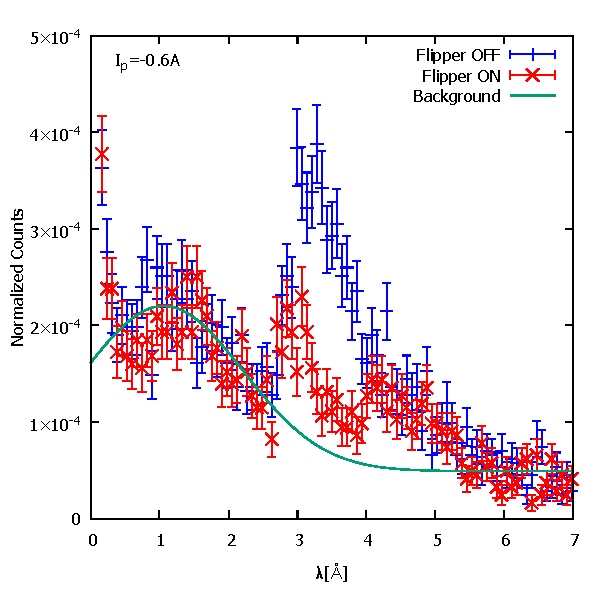
\includegraphics[width=5cm]{discussion/NC/NormalizedCounts_-6A.pdf}
\end{minipage}
\begin{minipage}{0.33\hsize}
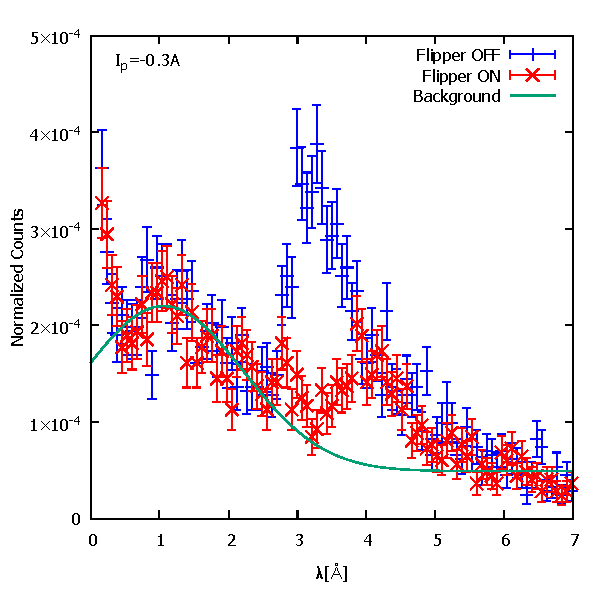
\includegraphics[width=5cm]{discussion/NC/NormalizedCounts_-3A.pdf}
\end{minipage}\\
\begin{minipage}{0.33\hsize}
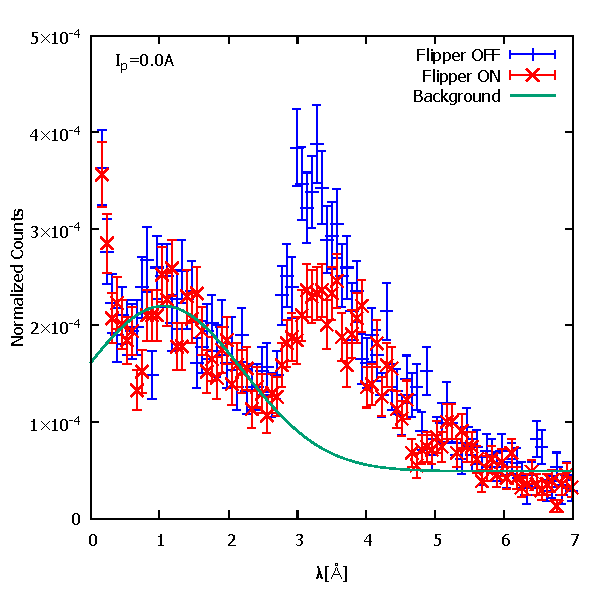
\includegraphics[width=5cm]{discussion/NC/NormalizedCounts_0A.pdf}
\end{minipage}
\begin{minipage}{0.33\hsize}
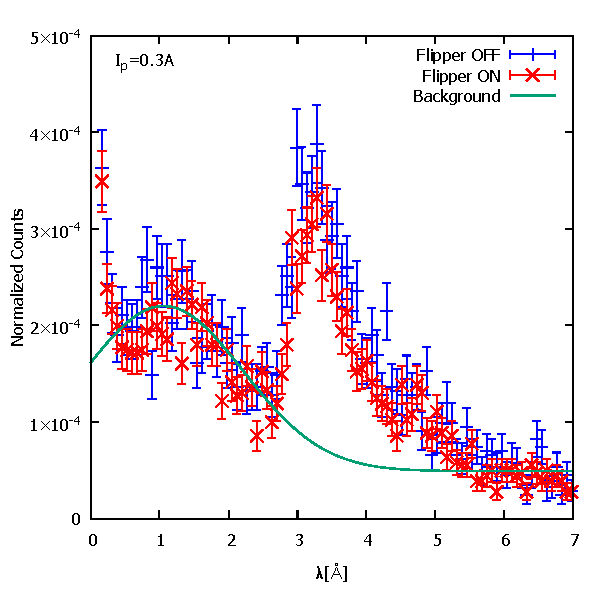
\includegraphics[width=5cm]{discussion/NC/NormalizedCounts_3A.pdf}
\end{minipage}
\begin{minipage}{0.33\hsize}
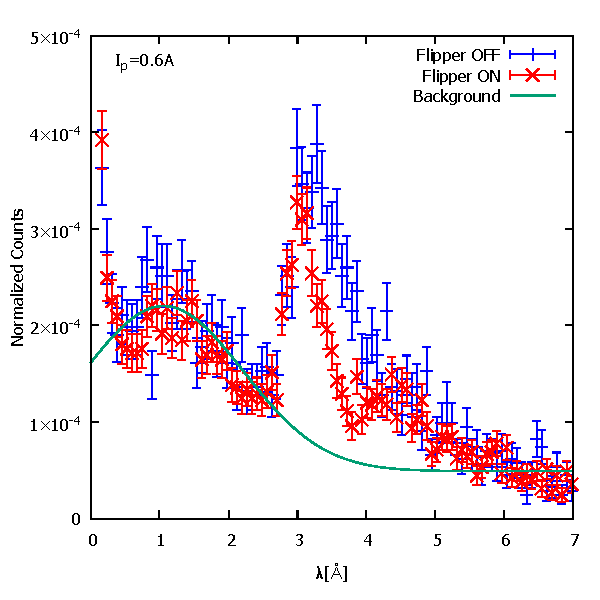
\includegraphics[width=5cm]{discussion/NC/NormalizedCounts_6A.pdf}
\end{minipage}\\
\begin{minipage}{0.33\hsize}
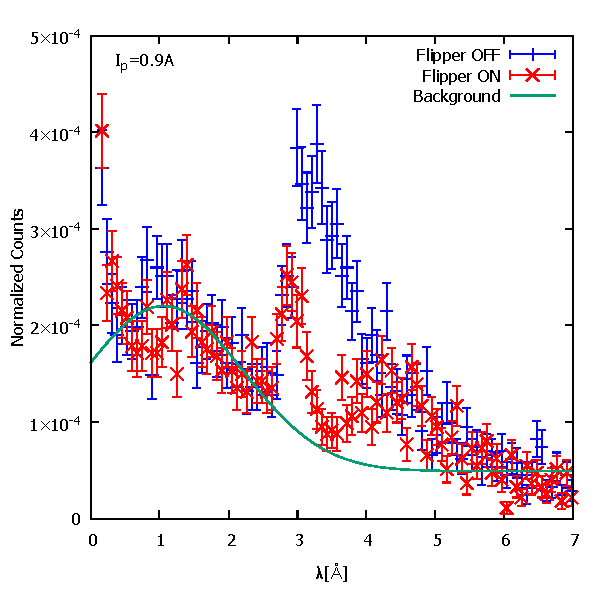
\includegraphics[width=5cm]{discussion/NC/NormalizedCounts_9A.pdf}
\end{minipage}
\begin{minipage}{0.33\hsize}
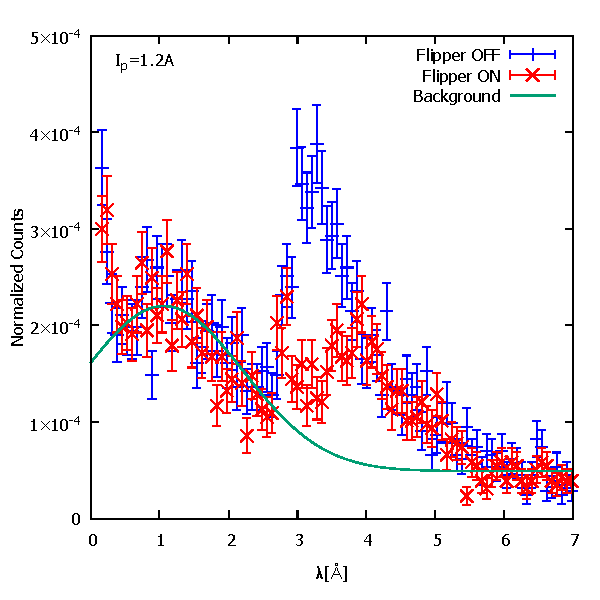
\includegraphics[width=5cm]{discussion/NC/NormalizedCounts_12A.pdf}
\end{minipage}
\begin{minipage}{0.33\hsize}
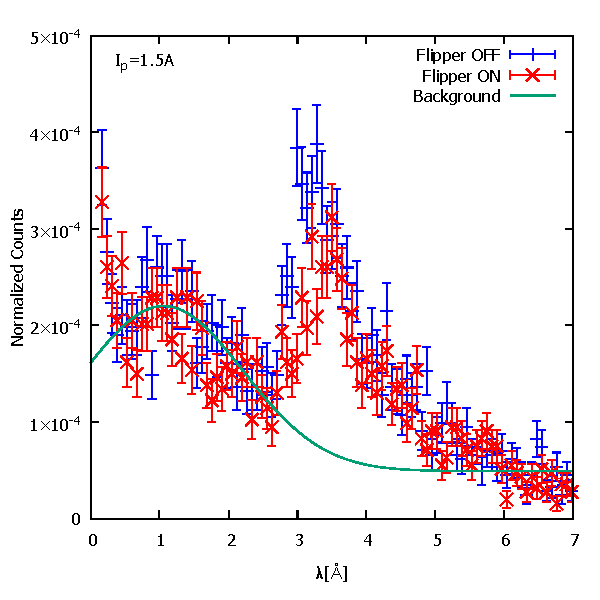
\includegraphics[width=5cm]{discussion/NC/NormalizedCounts_15A.pdf}
\end{minipage}\\
\begin{minipage}{0.33\hsize}
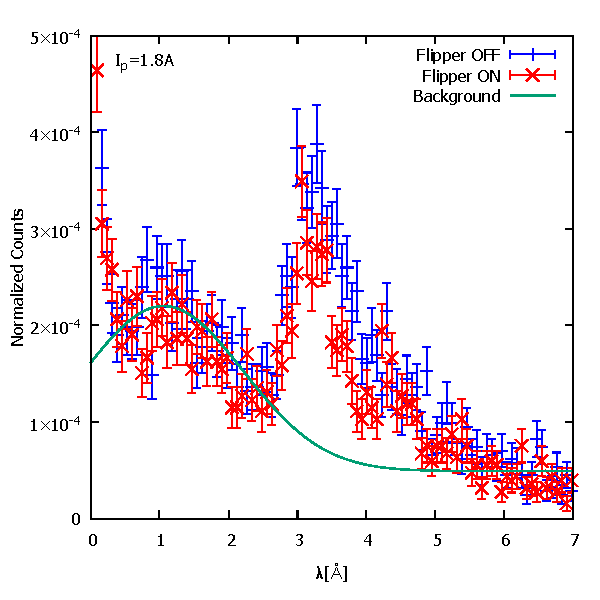
\includegraphics[width=5cm]{discussion/NC/NormalizedCounts_18A.pdf}
\end{minipage}
\begin{minipage}{0.33\hsize}
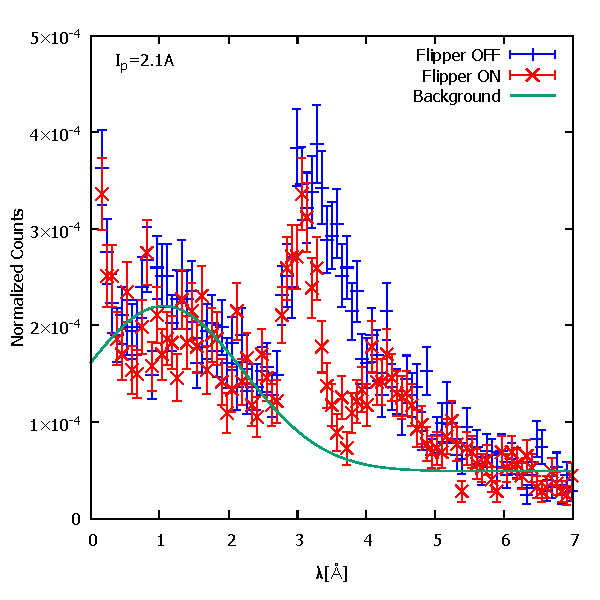
\includegraphics[width=5cm]{discussion/NC/NormalizedCounts_21A.pdf}
\end{minipage}
\begin{minipage}{0.33\hsize}
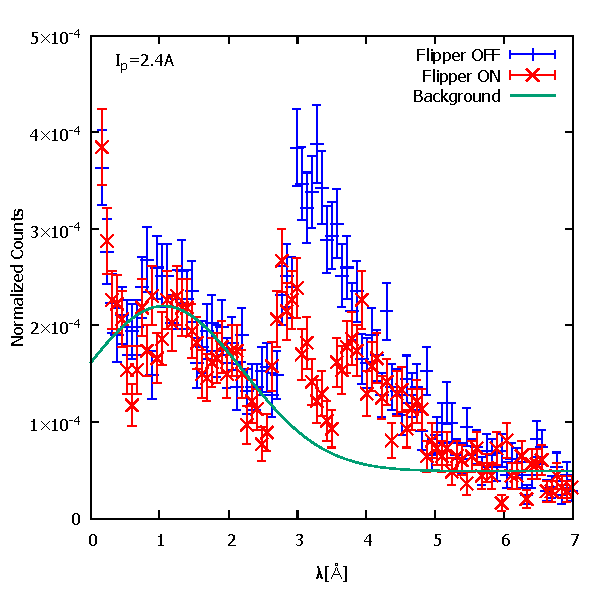
\includegraphics[width=5cm]{discussion/NC/NormalizedCounts_24A.pdf}
\end{minipage}
\caption{規格化粒子数の波長分布(バックグラウンドを引く前)}\label{Discussion_fig_NC}
\end{figure}

\begin{figure}[h]
\begin{minipage}{0.33\hsize}
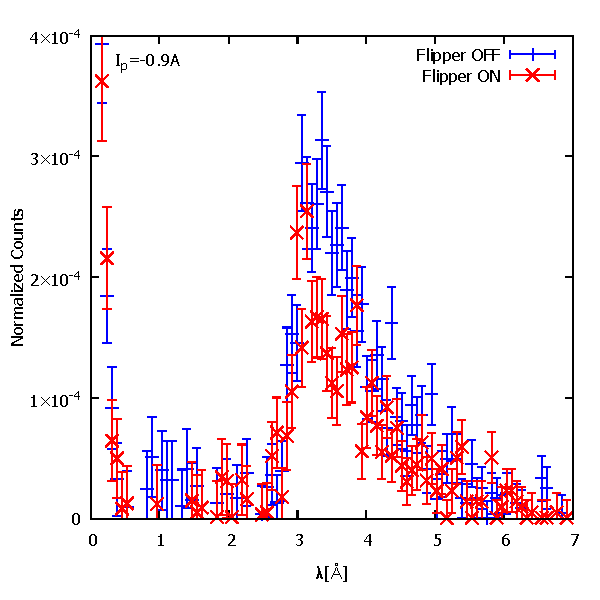
\includegraphics[width=5cm]{discussion/NC-BG/NormalizedCounts_b_-9A.pdf}
\end{minipage}
\begin{minipage}{0.33\hsize}
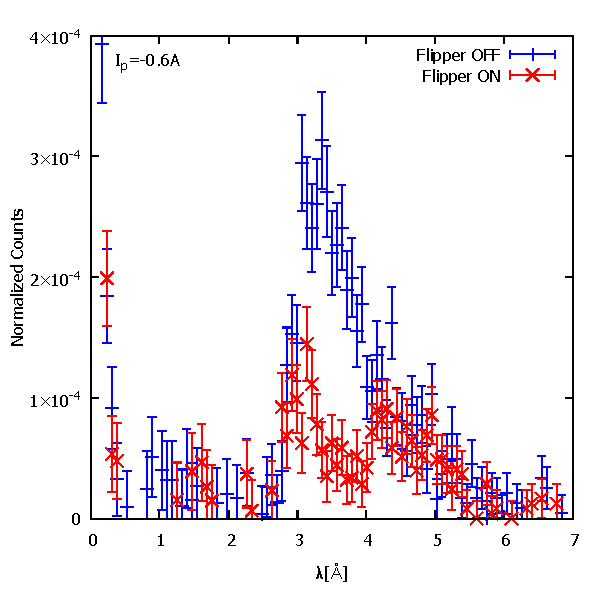
\includegraphics[width=5cm]{discussion/NC-BG/NormalizedCounts_b_-6A.pdf}
\end{minipage}
\begin{minipage}{0.33\hsize}
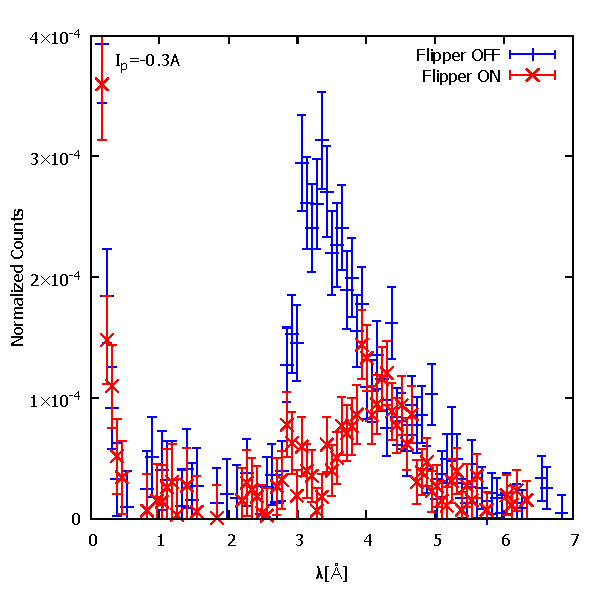
\includegraphics[width=5cm]{discussion/NC-BG/NormalizedCounts_b_-3A.pdf}
\end{minipage}\\
\begin{minipage}{0.33\hsize}
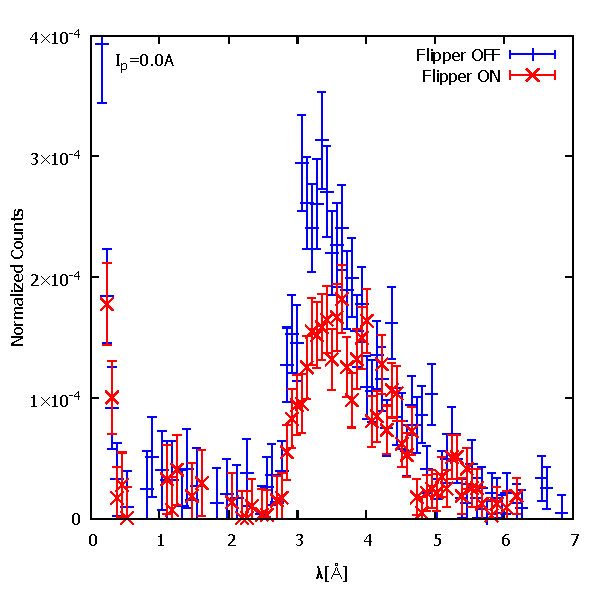
\includegraphics[width=5cm]{discussion/NC-BG/NormalizedCounts_b_0A.pdf}
\end{minipage}
\begin{minipage}{0.33\hsize}
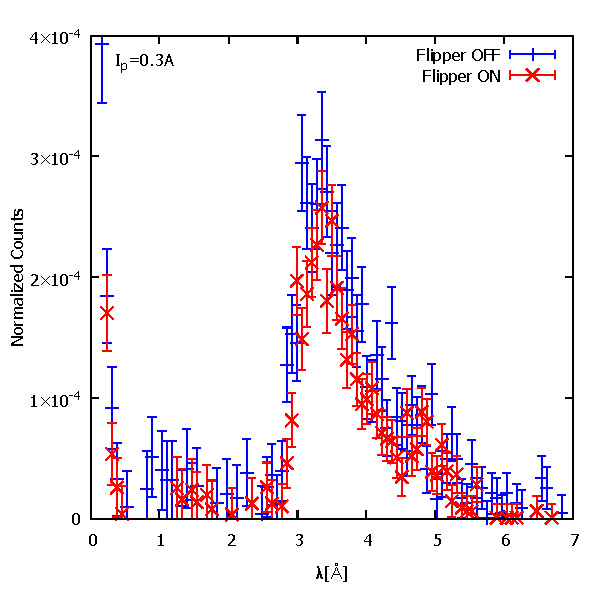
\includegraphics[width=5cm]{discussion/NC-BG/NormalizedCounts_b_3A.pdf}
\end{minipage}
\begin{minipage}{0.33\hsize}
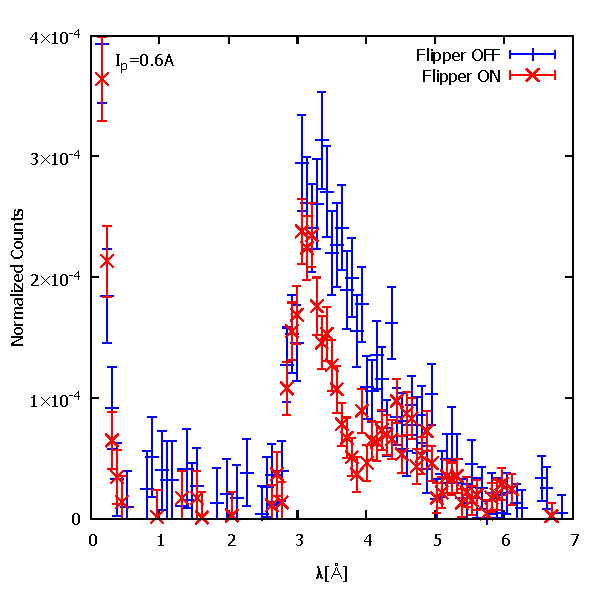
\includegraphics[width=5cm]{discussion/NC-BG/NormalizedCounts_b_6A.pdf}
\end{minipage}\\
\begin{minipage}{0.33\hsize}
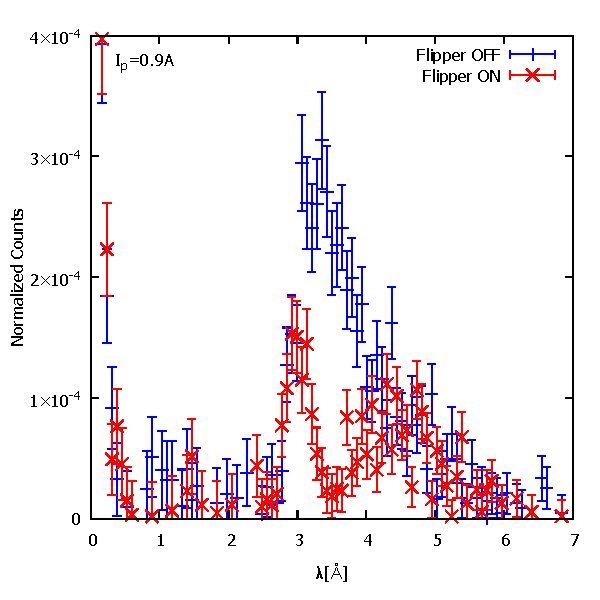
\includegraphics[width=5cm]{discussion/NC-BG/NormalizedCounts_b_9A.pdf}
\end{minipage}
\begin{minipage}{0.33\hsize}
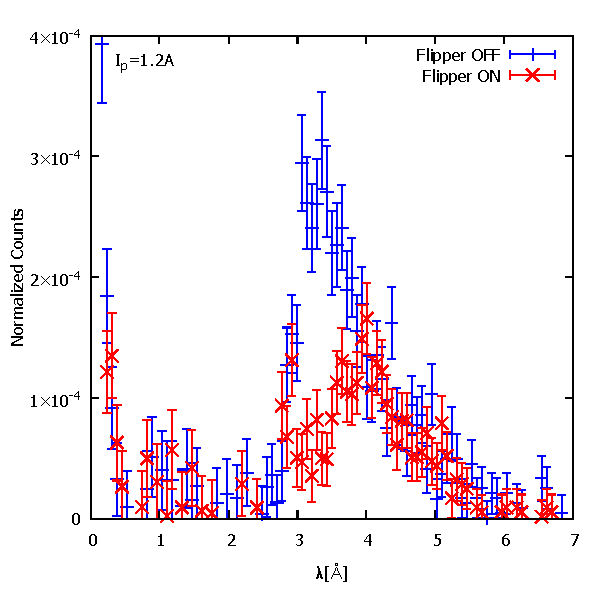
\includegraphics[width=5cm]{discussion/NC-BG/NormalizedCounts_b_12A.pdf}
\end{minipage}
\begin{minipage}{0.33\hsize}
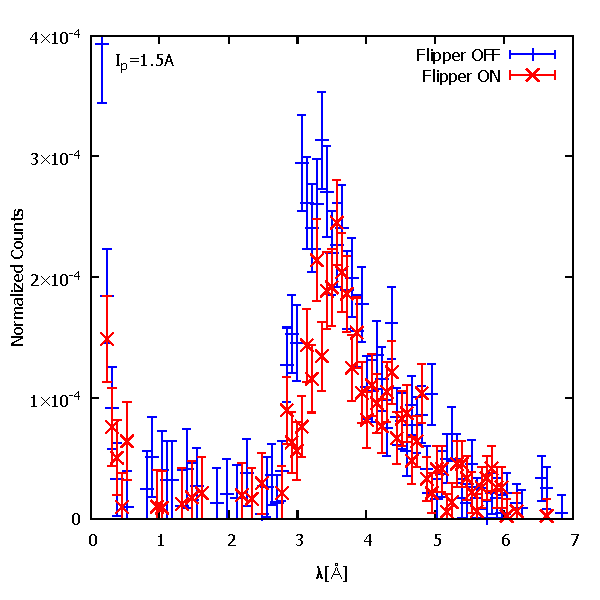
\includegraphics[width=5cm]{discussion/NC-BG/NormalizedCounts_b_15A.pdf}
\end{minipage}\\
\begin{minipage}{0.33\hsize}
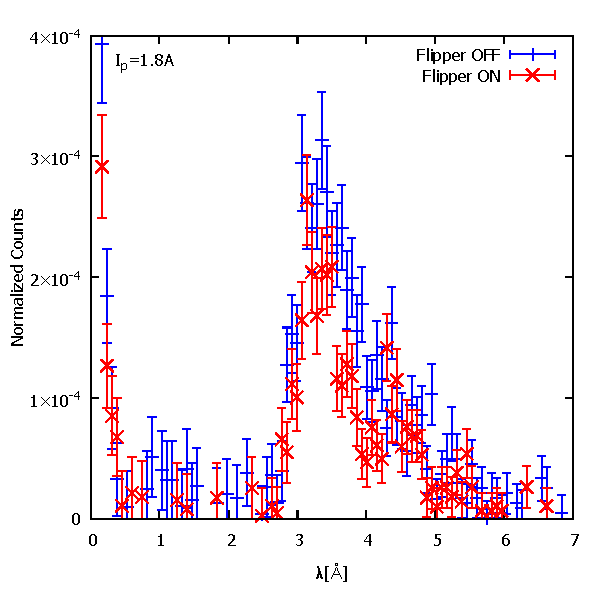
\includegraphics[width=5cm]{discussion/NC-BG/NormalizedCounts_b_18A.pdf}
\end{minipage}
\begin{minipage}{0.33\hsize}
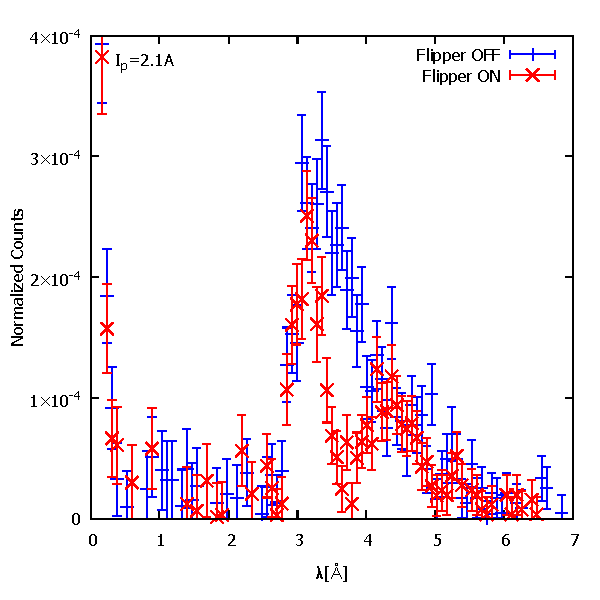
\includegraphics[width=5cm]{discussion/NC-BG/NormalizedCounts_b_21A.pdf}
\end{minipage}
\begin{minipage}{0.33\hsize}
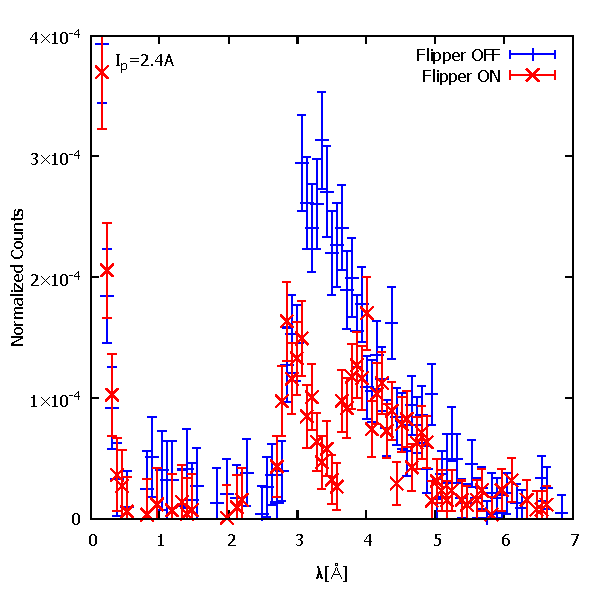
\includegraphics[width=5cm]{discussion/NC-BG/NormalizedCounts_b_24A.pdf}
\end{minipage}
\caption{規格化粒子数の波長分布(バックグラウンドを引いた後)}\label{Discussion_fig_NC_b}
\end{figure}

\begin{figure}[h]
\begin{minipage}{0.5\hsize}
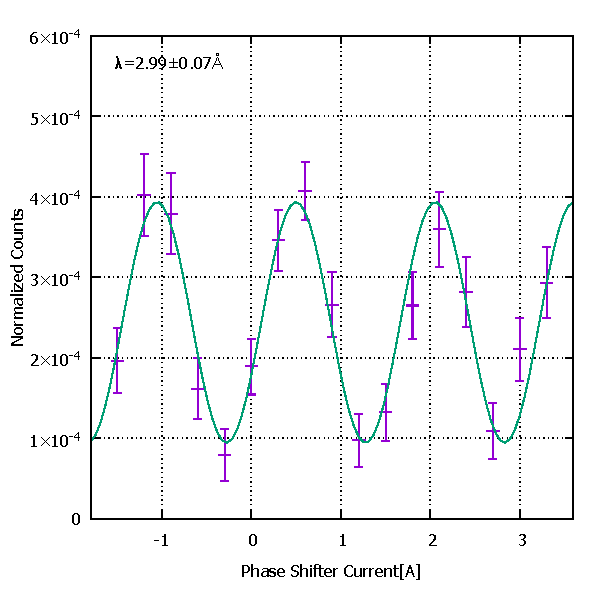
\includegraphics[width=\hsize]{discussion/IF_nb/Interference_nb_fit420.pdf}
\end{minipage}
\begin{minipage}{0.5\hsize}
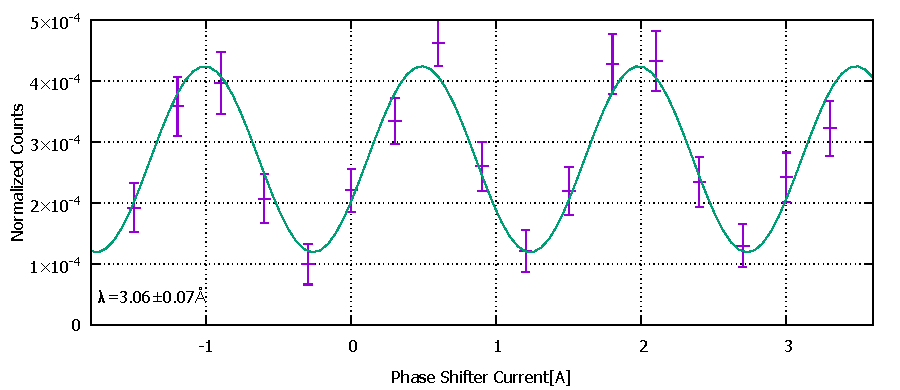
\includegraphics[width=\hsize]{discussion/IF_nb/Interference_nb_fit430.pdf}
\end{minipage}\\
\begin{minipage}{0.5\hsize}
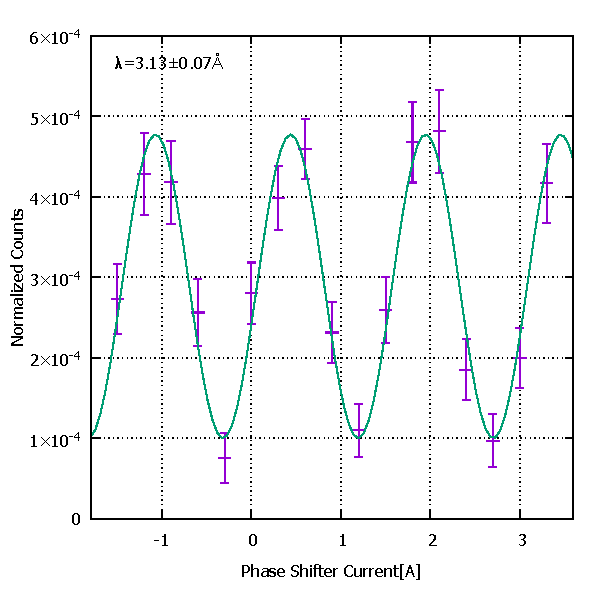
\includegraphics[width=\hsize]{discussion/IF_nb/Interference_nb_fit440.pdf}
\end{minipage}
\begin{minipage}{0.5\hsize}
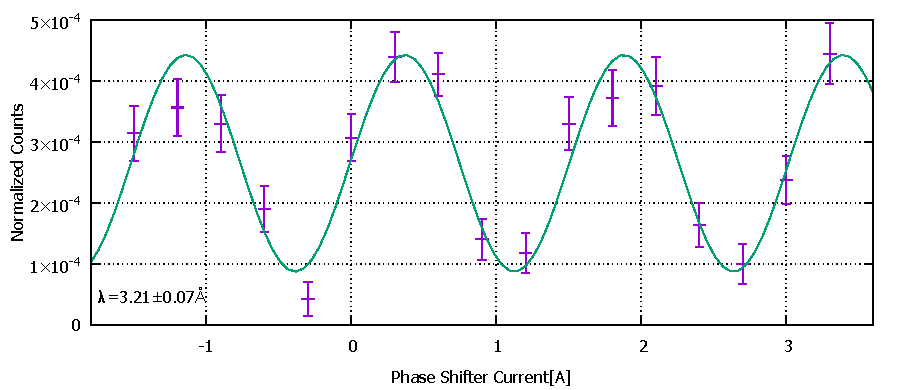
\includegraphics[width=\hsize]{discussion/IF_nb/Interference_nb_fit450.pdf}
\end{minipage}\\
\begin{minipage}{0.5\hsize}
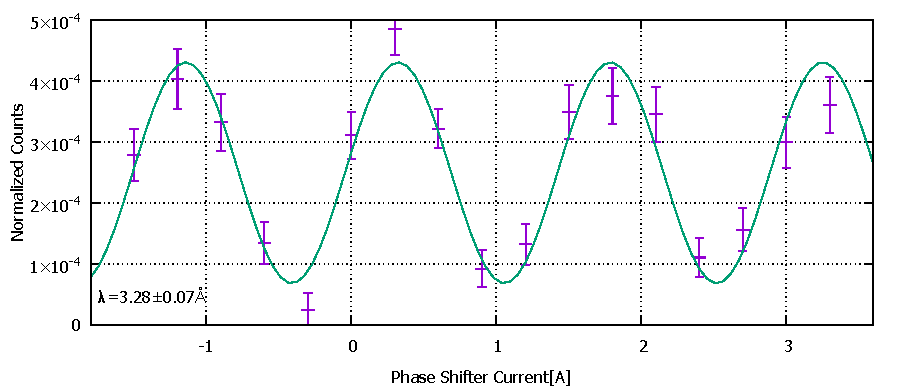
\includegraphics[width=\hsize]{discussion/IF_nb/Interference_nb_fit460.pdf}
\end{minipage}
\begin{minipage}{0.5\hsize}
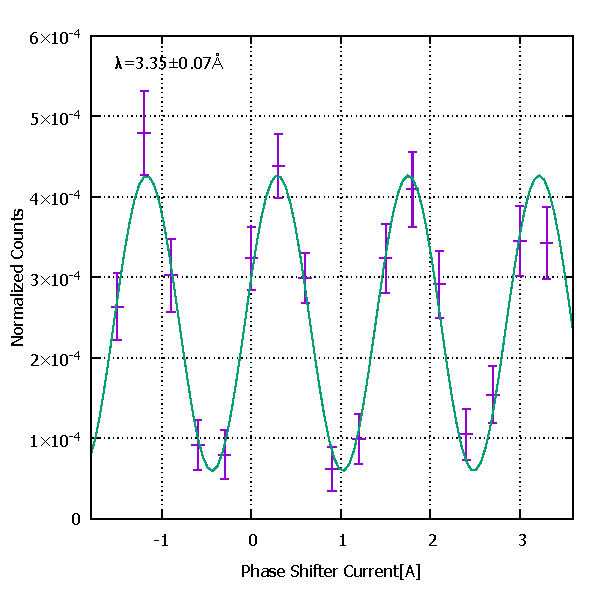
\includegraphics[width=\hsize]{discussion/IF_nb/Interference_nb_fit470.pdf}
\end{minipage}\\
\begin{minipage}{0.5\hsize}
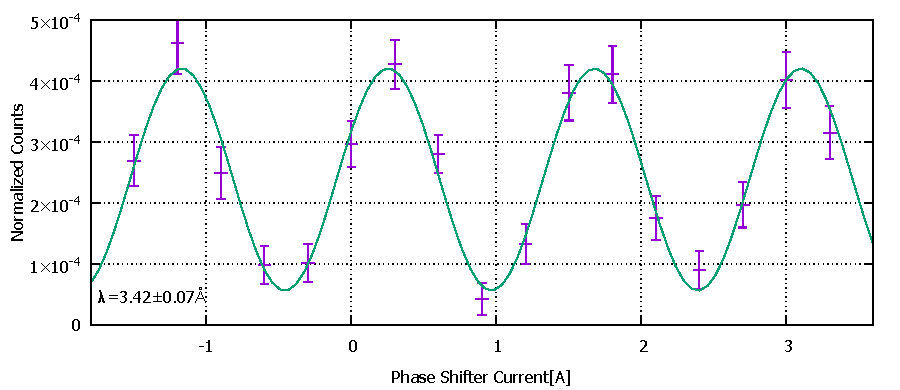
\includegraphics[width=\hsize]{discussion/IF_nb/Interference_nb_fit480.pdf}
\end{minipage}
\begin{minipage}{0.5\hsize}
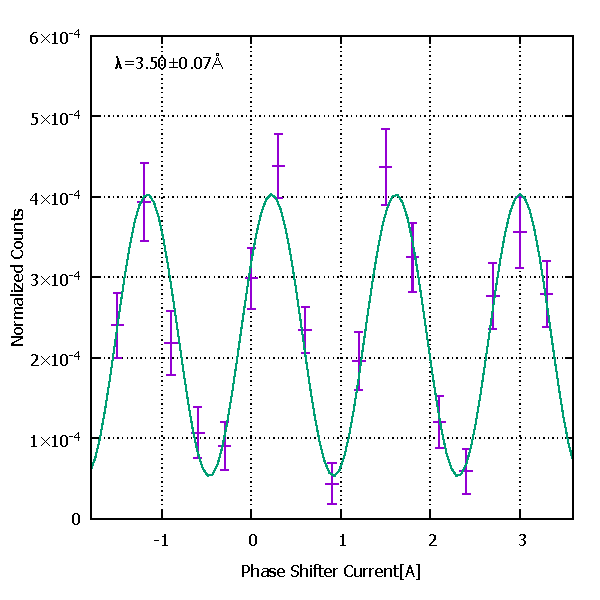
\includegraphics[width=\hsize]{discussion/IF_nb/Interference_nb_fit490.pdf}
\end{minipage}\\
\begin{minipage}{0.5\hsize}
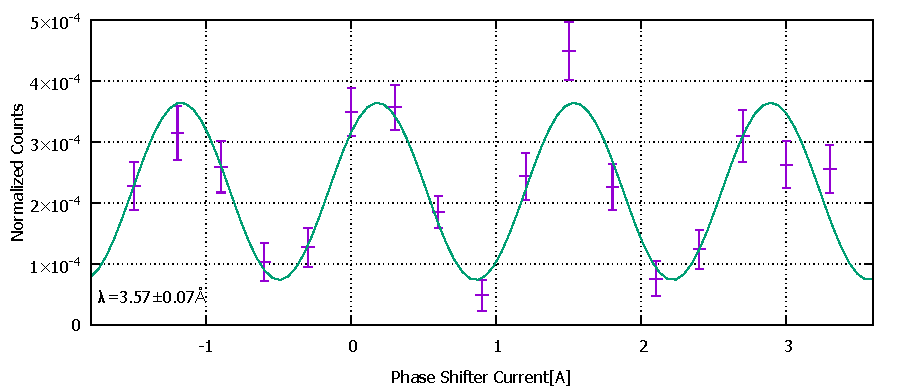
\includegraphics[width=\hsize]{discussion/IF_nb/Interference_nb_fit500.pdf}
\end{minipage}
\begin{minipage}{0.5\hsize}
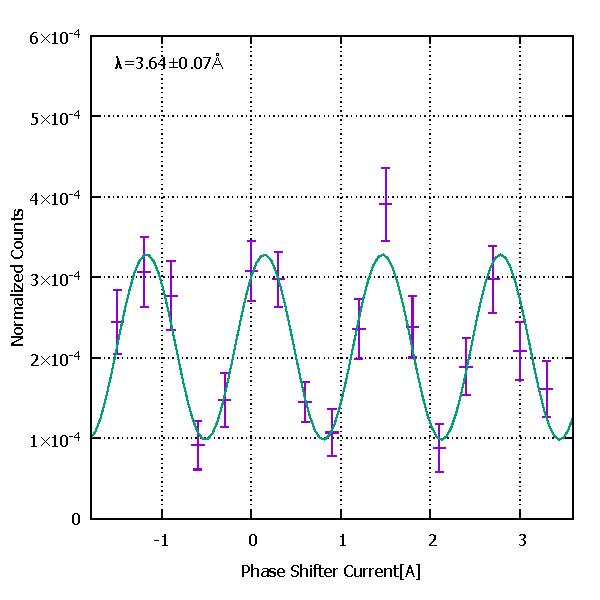
\includegraphics[width=\hsize]{discussion/IF_nb/Interference_nb_fit510.pdf}
\end{minipage}\\
\begin{minipage}{0.5\hsize}
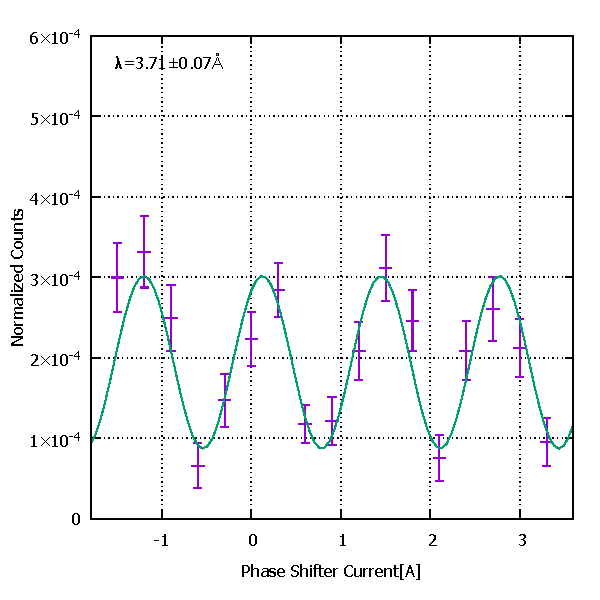
\includegraphics[width=\hsize]{discussion/IF_nb/Interference_nb_fit520.pdf}
\end{minipage}
\begin{minipage}{0.5\hsize}
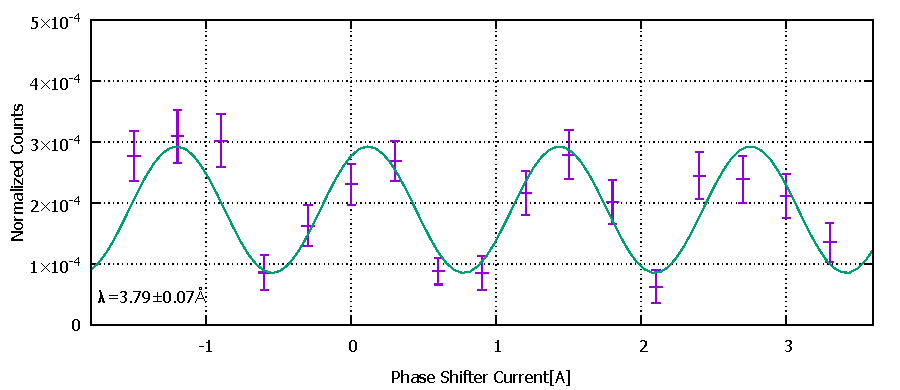
\includegraphics[width=\hsize]{discussion/IF_nb/Interference_nb_fit530.pdf}
\end{minipage}
\caption{規格化粒子数の干渉パターン}\label{Discussion_fig_IF_nb}
\end{figure}

\begin{figure}[h]
\begin{minipage}{0.5\hsize}
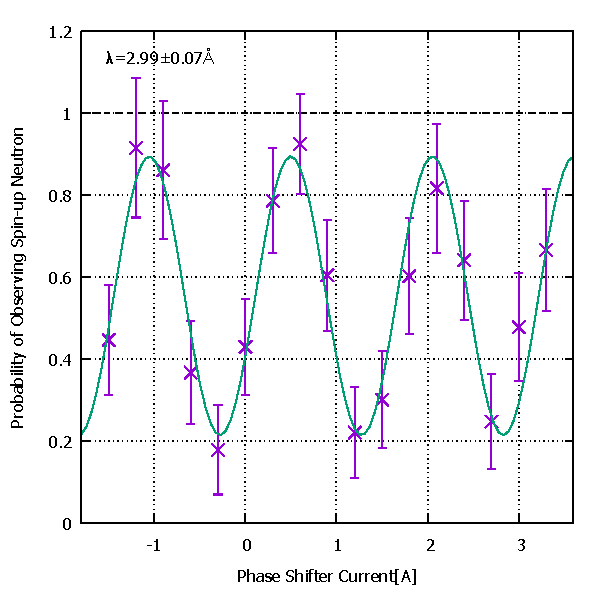
\includegraphics[width=\hsize]{discussion/IF_rb/Interference_rb_fit420.pdf}
\end{minipage}
\begin{minipage}{0.5\hsize}
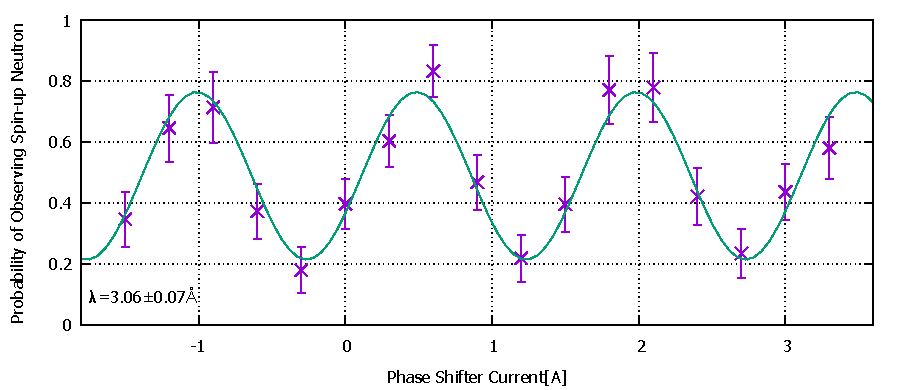
\includegraphics[width=\hsize]{discussion/IF_rb/Interference_rb_fit430.pdf}
\end{minipage}\\
\begin{minipage}{0.5\hsize}
\includegraphics[width=\hsize]{discussion/IF_rb/Interference_rb_fit440.pdf}
\end{minipage}
\begin{minipage}{0.5\hsize}
\includegraphics[width=\hsize]{discussion/IF_rb/Interference_rb_fit450.pdf}
\end{minipage}\\
\begin{minipage}{0.5\hsize}
\includegraphics[width=\hsize]{discussion/IF_rb/Interference_rb_fit460.pdf}
\end{minipage}
\begin{minipage}{0.5\hsize}
\includegraphics[width=\hsize]{discussion/IF_rb/Interference_rb_fit470.pdf}
\end{minipage}\\
\begin{minipage}{0.5\hsize}
\includegraphics[width=\hsize]{discussion/IF_rb/Interference_rb_fit480.pdf}
\end{minipage}
\begin{minipage}{0.5\hsize}
\includegraphics[width=\hsize]{discussion/IF_rb/Interference_rb_fit490.pdf}
\end{minipage}\\
\begin{minipage}{0.5\hsize}
\includegraphics[width=\hsize]{discussion/IF_rb/Interference_rb_fit500.pdf}
\end{minipage}
\begin{minipage}{0.5\hsize}
\includegraphics[width=\hsize]{discussion/IF_rb/Interference_rb_fit510.pdf}
\end{minipage}\\
\begin{minipage}{0.5\hsize}
\includegraphics[width=\hsize]{discussion/IF_rb/Interference_rb_fit520.pdf}
\end{minipage}
\begin{minipage}{0.5\hsize}
\includegraphics[width=\hsize]{discussion/IF_rb/Interference_rb_fit530.pdf}
\end{minipage}
\caption{スピン上向き中性子観測確率の干渉パターン}\label{Discussion_fig_IF_rb}
\end{figure}

\clearpage
\begin{table}[h]
\centering
\caption{各中心波長$\lambda$に対するパラメータ$A, B, C, D$とreduced$\chi^2$}\label{Discussion_tbl_IF_rb}
\begin{tabular}{cccccc}
$\lambda$[\AA]&$A$&$B$&$C$&$D$&reduced$\chi^2$\\ \hline
2.92 	&	0.36 	$\pm$	0.07 	&	3.84 	$\pm$	0.07 	&	0.92 	$\pm$	0.13 	&	0.76 	$\pm$	0.12 	&	0.78 	\\
2.99 	&	0.34 	$\pm$	0.05 	&	4.04 	$\pm$	0.05 	&	1.13 	$\pm$	0.09 	&	0.55 	$\pm$	0.07 	&	0.80 	\\
3.06 	&	0.27 	$\pm$	0.03 	&	4.20 	$\pm$	0.05 	&	1.11 	$\pm$	0.09 	&	0.49 	$\pm$	0.05 	&	0.75 	\\
3.13 	&	0.38 	$\pm$	0.05 	&	4.16 	$\pm$	0.04 	&	1.32 	$\pm$	0.07 	&	0.58 	$\pm$	0.06 	&	0.66 	\\
3.21 	&	0.36 	$\pm$	0.05 	&	4.16 	$\pm$	0.06 	&	1.61 	$\pm$	0.10 	&	0.53 	$\pm$	0.06 	&	1.26 	\\
3.28 	&	0.32 	$\pm$	0.04 	&	4.29 	$\pm$	0.06 	&	1.76 	$\pm$	0.10 	&	0.43 	$\pm$	0.05 	&	1.33 	\\
3.35 	&	0.31 	$\pm$	0.03 	&	4.29 	$\pm$	0.04 	&	1.89 	$\pm$	0.06 	&	0.42 	$\pm$	0.04 	&	0.58 	\\
3.42 	&	0.37 	$\pm$	0.04 	&	4.41 	$\pm$	0.04 	&	2.03 	$\pm$	0.06 	&	0.49 	$\pm$	0.05 	&	0.58 	\\
3.50 	&	0.39 	$\pm$	0.05 	&	4.52 	$\pm$	0.04 	&	2.13 	$\pm$	0.07 	&	0.51 	$\pm$	0.06 	&	0.80 	\\
3.57 	&	0.31 	$\pm$	0.05 	&	4.63 	$\pm$	0.07 	&	2.31 	$\pm$	0.11 	&	0.47 	$\pm$	0.05 	&	1.39 	\\
3.64 	&	0.27 	$\pm$	0.04 	&	4.76 	$\pm$	0.06 	&	2.45 	$\pm$	0.10 	&	0.49 	$\pm$	0.06 	&	0.70 	\\
3.71 	&	0.28 	$\pm$	0.05 	&	4.74 	$\pm$	0.09 	&	2.56 	$\pm$	0.15 	&	0.50 	$\pm$	0.06 	&	1.30 	\\
3.79 	&	0.29 	$\pm$	0.05 	&	4.76 	$\pm$	0.11 	&	2.60 	$\pm$	0.17 	&	0.53 	$\pm$	0.07 	&	1.64 	\\
3.86 	&	0.23 	$\pm$	0.04 	&	5.06 	$\pm$	0.10 	&	2.89 	$\pm$	0.16 	&	0.57 	$\pm$	0.08 	&	0.84 	\\
3.93 	&	0.29 	$\pm$	0.07 	&	5.02 	$\pm$	0.13 	&	3.44 	$\pm$	0.22 	&	0.65 	$\pm$	0.10 	&	1.72 	\\
4.00 	&	0.32 	$\pm$	0.07 	&	5.13 	$\pm$	0.08 	&	3.12 	$\pm$	0.14 	&	0.87 	$\pm$	0.15 	&	0.48 	\\ \hline
\end{tabular}
\end{table}

\paragraph{解析・考察}
バックグラウンドを考慮することによって各パラメータはどのように変わり変わらなかったのか分析を行い、その理由を考察する。
表\ref{Discussion_tbl_ABCDb}にパラメータ$A, B, C, D$のバックグラウンド考慮前、考慮後の実験値と理論値をそれぞれ示し、その結果を図\ref{Discussion_fig_ABCDb}に表す。表\ref{Discussion_tbl_ABCDb}と図\ref{Discussion_fig_ABCDb}から次のことが考察できる。
\begin{itemize}
\item パラメータ$B, C$は位相に関係した量であるからバックグラウンドによる影響はほぼなく、バックグラウンドを考慮する前と後で有効数字の範囲では誤差も含めて全く変化しない。したがって実験値と理論値はよく一致したまま保たれる。
\item パラメータ$D$は波の水深に関係する量であるからバックグラウンドの影響を受ける。バックグラウンドを考慮すると全体に小さくなる方へシフトし、3.0-3.8\AA の領域では実験値と理論値はよく一致する。領域の外では実験値が理論値よりも上へとずれてゆく。これは波長3\AA 以下や4\AA 以上では反射中性子の数が少なくなるため、下で述べるような粒子数を変化させる他の要因に強く影響されるためと考えられる。
\item パラメータ$A$も$D$と同じく波の水深に関係する量であるからバックグラウンドの影響を受ける。バックグラウンドを考慮すると、理論で予想されるまでには届かないものの、全体に上へシフトする。パラメータ$A$は位相の影響も受け、$\pm 0.07$\AA の波長領域で積分すると理論値は最大4\% 程度小さくなることを考慮すれば、理論値と実験値はさらに近づく。このようにパラメータ$A$は様々な影響を複合的に受けるためずれの原因をつきとめるのは困難であるが、次に述べるような粒子数を変化させる他の要因にも大きく影響されると考えられる。
\item 粒子数を変化させる他の要因としては、不均一磁場による軌道の変化や、空気によるスピンの反転、地磁気などの外部磁場によるスピンの反転などが考えられるが定量的な議論は難しい。
\end{itemize}

\begin{table}[H]
\caption{バックグラウンド考慮前後における実験値と理論値}\label{Discussion_tbl_ABCDb}
\begin{minipage}{0.5\hsize}
\subcaption{$A$}
\centering
\begin{tabular}{cccc}
$\lambda$[\AA]&BG考慮前&BG考慮後&理論値\\ \hline
2.92&0.21$\pm$0.03&0.36$\pm$0.07&0.44\\
2.99 	&	0.24 	$\pm$	0.03 	&	0.34 	$\pm$	0.05 	&	0.45 	\\
3.06 	&	0.21 	$\pm$	0.02 	&	0.27 	$\pm$	0.03 	&	0.46 	\\
3.13 	&	0.28 	$\pm$	0.03 	&	0.38 	$\pm$	0.05 	&	0.47 	\\
3.21 	&	0.27 	$\pm$	0.03 	&	0.36 	$\pm$	0.05 	&	0.47 	\\
3.28 	&	0.25 	$\pm$	0.03 	&	0.32 	$\pm$	0.04 	&	0.48 	\\
3.35 	&	0.25 	$\pm$	0.02 	&	0.31 	$\pm$	0.03 	&	0.48 	\\
3.42 	&	0.29 	$\pm$	0.03 	&	0.37 	$\pm$	0.04 	&	0.49 	\\
3.50 	&	0.30 	$\pm$	0.03 	&	0.39 	$\pm$	0.05 	&	0.49 	\\
3.57 	&	0.24 	$\pm$	0.03 	&	0.31 	$\pm$	0.05 	&	0.49 	\\
3.64 	&	0.21 	$\pm$	0.03 	&	0.27 	$\pm$	0.04 	&	0.50 	\\
3.71 	&	0.21 	$\pm$	0.03 	&	0.28 	$\pm$	0.05 	&	0.50 	\\
3.79 	&	0.22 	$\pm$	0.04 	&	0.29 	$\pm$	0.05 	&	0.50 	\\
3.86 	&	0.17 	$\pm$	0.03 	&	0.23 	$\pm$	0.04 	&	0.50 	\\
3.93 	&	0.21 	$\pm$	0.04 	&	0.29 	$\pm$	0.07 	&	0.50 	\\
4.00 	&	0.21 	$\pm$	0.03 	&	0.32 	$\pm$	0.07 	&	0.50	\\ \hline
\end{tabular}
\vspace{5mm}
\end{minipage}
\begin{minipage}{0.5\hsize}
\subcaption{$B$}
\centering
\begin{tabular}{cccc}
$\lambda$[\AA]&BG考慮前&BG考慮後&理論値\\ \hline
2.92&3.84$\pm$0.07&3.84$\pm$0.07&3.71\\
2.99 	&	4.04 	$\pm$	0.05 	&	4.04 	$\pm$	0.05 	&	3.81 	\\
3.06 	&	4.20 	$\pm$	0.05 	&	4.20 	$\pm$	0.05 	&	3.90 	\\
3.13 	&	4.16 	$\pm$	0.04 	&	4.16 	$\pm$	0.04 	&	3.99 	\\
3.21 	&	4.16 	$\pm$	0.06 	&	4.16 	$\pm$	0.06 	&	4.08 	\\
3.28 	&	4.29 	$\pm$	0.06 	&	4.29 	$\pm$	0.06 	&	4.18 	\\
3.35 	&	4.29 	$\pm$	0.04 	&	4.29 	$\pm$	0.04 	&	4.27 	\\
3.42 	&	4.41 	$\pm$	0.04 	&	4.41 	$\pm$	0.04 	&	4.36 	\\
3.50 	&	4.52 	$\pm$	0.04 	&	4.52 	$\pm$	0.04 	&	4.45 	\\
3.57 	&	4.63 	$\pm$	0.07 	&	4.63 	$\pm$	0.07 	&	4.54 	\\
3.64 	&	4.76 	$\pm$	0.06 	&	4.76 	$\pm$	0.06 	&	4.64 	\\
3.71 	&	4.74 	$\pm$	0.09 	&	4.74 	$\pm$	0.09 	&	4.73 	\\
3.79 	&	4.76 	$\pm$	0.11 	&	4.76 	$\pm$	0.11 	&	4.82 	\\
3.86 	&	5.06 	$\pm$	0.10 	&	5.06 	$\pm$	0.10 	&	4.91 	\\
3.93 	&	5.02 	$\pm$	0.13 	&	5.02 	$\pm$	0.13 	&	5.01 	\\
4.00 	&	5.13 	$\pm$	0.08 	&	5.13 	$\pm$	0.08 	&	5.10 	\\ \hline
\end{tabular}
\vspace{5mm}
\end{minipage}\\
\begin{minipage}{0.5\hsize}
\subcaption{$C$}
\centering
\begin{tabular}{cccc}
$\lambda$[\AA]&BG考慮前&BG考慮後&理論値\\ \hline
2.92&0.92$\pm$0.13&0.92$\pm$0.13&0.71\\
2.99 	&	1.13 	$\pm$	0.09 	&	1.13 	$\pm$	0.09 	&	0.89 	\\
3.06 	&	1.11 	$\pm$	0.09 	&	1.11 	$\pm$	0.09 	&	1.07 	\\
3.13 	&	1.32 	$\pm$	0.07 	&	1.32 	$\pm$	0.07 	&	1.25 	\\
3.21 	&	1.61 	$\pm$	0.10 	&	1.61 	$\pm$	0.10 	&	1.43 	\\
3.28 	&	1.76 	$\pm$	0.10 	&	1.76 	$\pm$	0.10 	&	1.61 	\\
3.35 	&	1.89 	$\pm$	0.06 	&	1.89 	$\pm$	0.06 	&	1.80 	\\
3.42 	&	2.03 	$\pm$	0.06 	&	2.03 	$\pm$	0.06 	&	1.98 	\\
3.50 	&	2.13 	$\pm$	0.07 	&	2.13 	$\pm$	0.07 	&	2.17 	\\
3.57 	&	2.31 	$\pm$	0.11 	&	2.31 	$\pm$	0.11 	&	2.35 	\\
3.64 	&	2.45 	$\pm$	0.10 	&	2.45 	$\pm$	0.10 	&	2.54 	\\
3.71 	&	2.56 	$\pm$	0.15 	&	2.56 	$\pm$	0.15 	&	2.72 	\\
3.79 	&	2.60 	$\pm$	0.17 	&	2.60 	$\pm$	0.17 	&	2.91 	\\
3.86 	&	2.89 	$\pm$	0.16 	&	2.89 	$\pm$	0.16 	&	3.10 	\\
3.93 	&	3.44 	$\pm$	0.22 	&	3.44 	$\pm$	0.22 	&	3.29 	\\
4.00 	&	3.12 	$\pm$	0.14 	&	3.12 	$\pm$	0.14 	&	3.48 	\\ \hline
\end{tabular}
\end{minipage}
\begin{minipage}{0.5\hsize}
\subcaption{$D$}
\centering
\begin{tabular}{cccc}
$\lambda$[\AA]&BG考慮前&BG考慮後&理論値\\ \hline
2.92&0.85$\pm$0.08&0.76$\pm$0.12&0.55\\
2.99 	&	0.69 	$\pm$	0.06 	&	0.55 	$\pm$	0.07 	&	0.54 	\\
3.06 	&	0.61 	$\pm$	0.05 	&	0.49 	$\pm$	0.05 	&	0.54 	\\
3.13 	&	0.68 	$\pm$	0.05 	&	0.58 	$\pm$	0.06 	&	0.53 	\\
3.21 	&	0.64 	$\pm$	0.05 	&	0.53 	$\pm$	0.06 	&	0.52 	\\
3.28 	&	0.55 	$\pm$	0.04 	&	0.43 	$\pm$	0.05 	&	0.52 	\\
3.35 	&	0.53 	$\pm$	0.04 	&	0.42 	$\pm$	0.04 	&	0.51 	\\
3.42 	&	0.60 	$\pm$	0.05 	&	0.49 	$\pm$	0.05 	&	0.51 	\\
3.50 	&	0.62 	$\pm$	0.05 	&	0.51 	$\pm$	0.06 	&	0.50 	\\
3.57 	&	0.58 	$\pm$	0.05 	&	0.47 	$\pm$	0.05 	&	0.50 	\\
3.64 	&	0.61 	$\pm$	0.05 	&	0.49 	$\pm$	0.06 	&	0.50 	\\
3.71 	&	0.62 	$\pm$	0.06 	&	0.50 	$\pm$	0.06 	&	0.50 	\\
3.79 	&	0.65 	$\pm$	0.06 	&	0.53 	$\pm$	0.07 	&	0.50 	\\
3.86 	&	0.68 	$\pm$	0.07 	&	0.57 	$\pm$	0.08 	&	0.50 	\\
3.93 	&	0.75 	$\pm$	0.08 	&	0.65 	$\pm$	0.10 	&	0.50 	\\
4.00 	&	0.92 	$\pm$	0.10 	&	0.87 	$\pm$	0.15 	&	0.50 	\\ \hline
\end{tabular}
\end{minipage}
\end{table}

\begin{figure}[H]
\begin{center}
\includegraphics[width=12cm]{discussion/ABCD/A_ab.pdf}
\subcaption{$A$}
\vspace{1cm}
\includegraphics[width=12cm]{discussion/ABCD/B_ab.pdf}
\subcaption{$B$}
\end{center}
%\end{minipage}\\
%\begin{minipage}{0.5\hsize}
\caption{バックグラウンド考慮前後における実験値の比較}
\end{figure}
\begin{figure}[H]
\begin{center}
\ContinuedFloat
\includegraphics[width=12cm]{discussion/ABCD/C_ab_fit.pdf}
\subcaption{$C$}
\vspace{1cm}
\includegraphics[width=12cm]{discussion/ABCD/D_ab.pdf}
\subcaption{$D$}
\end{center}
\caption{バックグラウンド考慮前後における実験値の比較}\label{Discussion_fig_ABCDb}
%\end{minipage}
\end{figure}

\paragraph{波の合成}
バックグラウンドを考慮したときの波としての実験値と理論値を図\ref{Disucussion_BG_fig_IT_eb}に表す。
\begin{figure}[H]
\begin{minipage}{0.5\hsize}
\includegraphics[width=\hsize]{discussion/BG/IT_eb_420.pdf}
\end{minipage}
\begin{minipage}{0.5\hsize}
\includegraphics[width=\hsize]{discussion/BG/IT_eb_430.pdf}
\end{minipage}\\
\begin{minipage}{0.5\hsize}
\includegraphics[width=\hsize]{discussion/BG/IT_eb_440.pdf}
\end{minipage}
\begin{minipage}{0.5\hsize}
\includegraphics[width=\hsize]{discussion/BG/IT_eb_450.pdf}
\end{minipage}\\
\begin{minipage}{0.5\hsize}
\includegraphics[width=\hsize]{discussion/BG/IT_eb_460.pdf}
\end{minipage}
\begin{minipage}{0.5\hsize}
\includegraphics[width=\hsize]{discussion/BG/IT_eb_470.pdf}
\end{minipage}\\
\begin{minipage}{0.5\hsize}
\includegraphics[width=\hsize]{discussion/BG/IT_eb_480.pdf}
\end{minipage}
\begin{minipage}{0.5\hsize}
\includegraphics[width=\hsize]{discussion/BG/IT_eb_490.pdf}
\end{minipage}\\
\begin{minipage}{0.5\hsize}
\includegraphics[width=\hsize]{discussion/BG/IT_eb_500.pdf}
\end{minipage}
\begin{minipage}{0.5\hsize}
\includegraphics[width=\hsize]{discussion/BG/IT_eb_510.pdf}
\end{minipage}\\
\begin{minipage}{0.5\hsize}
\includegraphics[width=\hsize]{discussion/BG/IT_eb_520.pdf}
\end{minipage}
\begin{minipage}{0.5\hsize}
\includegraphics[width=\hsize]{discussion/BG/IT_eb_530.pdf}
\end{minipage}
\caption{干渉パターンのバックグラウンドを考慮した実験値と理論値}\label{Disucussion_BG_fig_IT_eb}
\end{figure}

\subsection{まとめ}
この章では波の水深に関係した2つのパラメータ$A, D$の実験結果を理論的に説明するべく、スピンフリッパー間の距離による効果とバックグラウンドによる影響の2つの仮説を立てた。前者はパラメータ$C$の実験結果に矛盾するという理由から棄却され、後者は全ての実験結果をよく説明した。

最後に、干渉波のうなりに関する美しい結果を紹介する。これまでは分解した要素と理論値を対応させるために狭い波長領域しか考えることができなかった。しかし波を波として捉えればどんな波長領域でも扱うことができる。中心波長$\lambda=3.42$\AA に対して領域$\pm 0.07, \pm0.14, \pm0.22, \pm0.29, \pm0.36, \pm0.43, \pm0.51$\AA を取ったときの実験値と理論値は次の図\ref{Discussion_fig_around480}のようになる。波長領域を広げることで位相のずれが大きくなり、干渉のうなりが生じる様子が実験値からはっきりと見て取れる。狭い波長領域でみたときに実験値と理論値はよく一致していたことから、広い波長領域でみても実験値と理論値は当然よく一致すべきではあるが、うなりによる振幅の変動を理論が精度よく予測している様子は非常に美しい。
\vspace{1cm}
\begin{figure}[H]
\centering
%\begin{minipage}{0.5\hsize}
\includegraphics[width=10cm]{discussion/SEA/IT_480_10.pdf}
%\end{minipage}
%\begin{minipage}{0.5\hsize}
\includegraphics[width=10cm]{discussion/SEA/IT_480_20.pdf}
%\end{minipage}\\
%\begin{minipage}{0.5\hsize}
\includegraphics[width=10cm]{discussion/SEA/IT_480_30.pdf}
%\end{minipage}
%\begin{minipage}{0.5\hsize}
\caption{広い波長領域における実験値と理論値}
\end{figure}
\begin{figure}[H]
\ContinuedFloat
\centering
%\end{minipage}\\
%\begin{minipage}{0.5\hsize}
\includegraphics[width=10cm]{discussion/SEA/IT_480_40.pdf}
\includegraphics[width=10cm]{discussion/SEA/IT_480_50.pdf}
%\end{minipage}
%\begin{minipage}{0.5\hsize}
\includegraphics[width=10cm]{discussion/SEA/IT_480_60.pdf}
%\end{minipage}\\
%\begin{minipage}{0.5\hsize}
\includegraphics[width=10cm]{discussion/SEA/IT_480_70.pdf}
%\end{minipage}
\caption{広い波長領域における実験値と理論値}\label{Discussion_fig_around480}
\end{figure}
